\documentclass[10pt, letterpaper]{report}
% !TeX program = xelatex
%==================PREAMBOLO=======================%
\usepackage[utf8]{inputenc}
\usepackage{psvectorian}
\usepackage{pgfplots}
\usepackage[Rejne]{fncychap}
\usepackage[export]{adjustbox}
\usepackage[T1]{fontenc}
\usepackage{lmodern}
\usepackage{blindtext}
\usepackage{pdfpages}
\usepackage[shortlabels]{enumitem}
\usepackage{moresize}
\usepackage{graphicx} % Required for inserting images
\usepackage{hyperref}
\usepackage{listings}
\usepackage[table,xcdraw]{xcolor}
\usepackage{amssymb}
\usepackage{amsmath}
\usepackage[english]{babel}
\usepackage{nicefrac, xfrac}
\usepackage{tikz}
\usepackage{tikz-3dplot}
\usepackage{tikz-cd}
\usepackage{mathrsfs} 
\usepackage{titletoc}
\usepackage{fancyhdr}
\usepackage{psvectorian,lipsum}
\usepackage{fourier-orns}
\usepackage{lipsum}
\usepackage{wrapfig}
\usepackage{multicol}
\usepackage[paper=a4paper,left=25mm,right=25mm,bottom=25mm,top=25mm]{geometry}
\definecolor{light-gray}{gray}{0.95}
\definecolor{cop}{HTML}{f7ecd7}
\definecolor{copAut}{HTML}{ababab}
\definecolor{copAut2}{HTML}{c3c3e6}
\definecolor{purcop}{HTML}{d0d3db}
\definecolor{sapienza}{HTML}{660f1d}
\definecolor{lightSapienza}{HTML}{e3d3d5}
\definecolor{darkgreen}{HTML}{008000}
\definecolor{cartaRiciclata}{HTML}{fcfcf7}
\newcommand{\redText}[1]{\color{red}#1\color{black}}
\newcommand{\code}[1]{\colorbox{light-gray}{\texttt{#1}}}
\newcommand{\codee}[1]{\colorbox{white}{\texttt{#1}}}
\newcommand{\K}{{\mathbb K}}
\newcommand{\notimplies}{%
  \mathrel{{\ooalign{\hidewidth$\not\phantom{=}$\hidewidth\cr$\implies$}}}}
\newcommand{\flowerLine}{ \begin{center}\decofourleft\hphantom{ }\decoone\hphantom{ }\decofourright\hphantom{}\hphantom{aa}
\decofourleft\hphantom{ }\decoone\hphantom{ }\decofourright\hphantom{}\hphantom{aa}
\decofourleft\hphantom{ }\decoone\hphantom{ }\decofourright\hphantom{}\hphantom{aa}
\decofourleft\hphantom{ }\decoone\hphantom{ }\decofourright\hphantom{}\hphantom{aa} 
\decofourleft\hphantom{ }\decoone\hphantom{ }\decofourright\hphantom{}\hphantom{aa}
\decofourleft\hphantom{ }\decoone\hphantom{ }\decofourright\hphantom{}\hphantom{aa}
\decofourleft\hphantom{ }\decoone\hphantom{ }\decofourright\hphantom{}\hphantom{aa}
\decofourleft\hphantom{ }\decoone\hphantom{ }\decofourright\hphantom{}\hphantom{aa}
\decofourleft\hphantom{ }\decoone\hphantom{ }\decofourright\hphantom{}\hphantom{aa}
\end{center}}
\definecolor{g}{RGB}{60, 50, 50}
\newcommand{\textg}[1]{\color{g}{\textbf{#1}}\color{black}}
\newcommand{\teo}[1]{{\large\color{sapienza}\textbf{Teorema #1 :\hphantom{a}}}}
\newcommand{\defi}[1]{{\large\color{sapienza}\textbf{Definizione #1 :\hphantom{a}}}}
\newcommand{\claim}[1]{{\color{sapienza}\textbf{Claim #1 :\hphantom{a}}}}
\newcommand{\lemma}[1]{{\color{sapienza}\textbf{Lemma #1 :\hphantom{a}}}}
\newcommand{\dimo}[1]{{\color{sapienza}\textbf{Dimostrazione #1 :\hphantom{a}}}}
\newcommand{\prop}[1]{{\color{sapienza}\textbf{Proposizione #1 :\hphantom{a}}}}
\newcommand\greybox[1]{%
  \vskip\baselineskip%
  \par\noindent\colorbox{light-gray}{%
    \begin{minipage}{\textwidth}#1\end{minipage}%
  }%
  \vskip\baselineskip%
}
\newcommand\sapbox[1]{%
  \vskip\baselineskip%
  \par\noindent\colorbox{lightSapienza}{%
    \begin{minipage}{\textwidth}#1\end{minipage}%
  }%
  \vskip\baselineskip%
}
\newcommand{\ridFunc}{{f:\Sigma^*\rightarrow \Sigma^*}}
\newcommand{\rid}{{\le_m^P}}
\newcommand{\Z}{{\mathbb Z}}
\newcommand{\blank}{{\sqcup}}
\newcommand{\Prob}{{\mathbb P}}
\newcommand{\R}{{\mathbb R}}
\newcommand{\VA}{{\mathbb E}}
\newcommand{\N}{{\mathbb N}}
\newcommand{\quat}{{\mathbb H}}
\newcommand{\C}{{\mathbb C}}
\newcommand{\Sn}{{\mathcal S_n}}
\newcommand{\An}{{\mathcal A_n}}
\newcommand{\E}{{\mathcal E}}
\newcommand{\B}{{\mathcal B}}
\newcommand{\mcm}{{\text{mcm}}}
\newcommand{\rg}{{\text{rg}}}
\newcommand{\ve}{{\bar v}}
\newcommand{\spaz}{{\text{\hphantom{aa}}}}
\newcommand{\MCD}{{\text{MCD}}}
\newcommand{\tc}{{\text{ tale che }}}
\newcommand{\supp}{{\text{Supp}}}
\newcommand{\acc}{\\\hphantom{}\\}
\newcommand{\esempio}[1]{{\acc\large\color{sapienza}\textbf{Esempio #1 \hphantom{a}}\acc}}
\newcommand{\bra}[1]{\langle #1 \rangle}
\newcommand{\aut}{{\text{Aut}}}
\newcommand{\Span}{{\text{Span}}}
\newcommand{\End}{{\text{End}}}
\newcommand{\cen}{{\text{Centro}}}
\newcommand{\norm}{{\unlhd}}
\newcommand{\ciclS}{{\left \langle }}
\newcommand{\ciclE}{{\right \rangle }}
\newcommand{\boxedMath}[1]{\begin{tabular}{|c|}\hline \texttt{#1} \\ \hline\end{tabular} :} 
\newcommand{\shell}[1]{\colorbox{black}{\textcolor{white}{\texttt{#1}}}}
\newcommand{\eqImportante}[1]{\begin{center}\huge\lefthand\hphantom{a}
    \normalsize\texttt{#1}
    \hphantom{aaa}\huge\righthand\end{center}}

\fancyhf{}
\pagestyle{fancy}
\usepackage{pgf-pie}  
\usetikzlibrary{positioning}

\renewcommand{\headrule}{%
\vspace{-8pt}\hrulefill
\raisebox{-2.1pt}{\quad\decothreeleft\decotwo\decothreeright\quad}\hrulefill}

%sta roba serve per il codice C
\definecolor{mGreen}{rgb}{0,0.6,0}
\definecolor{mGray}{rgb}{0.5,0.5,0.5}
\definecolor{mPurple}{rgb}{0.58,0,0.82}
\definecolor{backgroundColour}{rgb}{0.95,0.95,0.92}

\lstdefinestyle{CStyle}{
    backgroundcolor=\color{backgroundColour},   
    commentstyle=\color{mGreen},
    keywordstyle=\color{magenta},
    numberstyle=\tiny\color{mGray},
    stringstyle=\color{mPurple},
    basicstyle=\footnotesize,
    breakatwhitespace=false,         
    breaklines=true,                 
    captionpos=b,                    
    keepspaces=true,                 
    numbers=left,                    
    numbersep=5pt,                  
    showspaces=false,                
    showstringspaces=false,
    showtabs=false,                  
    tabsize=2,
    language=C
}
\lstdefinestyle{CppStyle}{
    backgroundcolor=\color{backgroundColour},   
    commentstyle=\color{mGreen}\ttfamily,
    morecomment=[l][\color{magenta}]{\#}
    keywordstyle=\color{blue}\ttfamily,
    numberstyle=\tiny\color{mGray},
    stringstyle=\color{red}\ttfamily,
    basicstyle=\ttfamily,
    breakatwhitespace=false,         
    breaklines=true,                 
    captionpos=b,                    
    keepspaces=true,                 
    numbers=left,                    
    numbersep=5pt,                  
    showspaces=false,                
    showstringspaces=false,
    showtabs=false,                  
    tabsize=2,
    language=C
}
\lstset{language=C++,
                basicstyle=\ttfamily,
                keywordstyle=\color{blue}\ttfamily,
                stringstyle=\color{red}\ttfamily,
                commentstyle=\color{green}\ttfamily,
                morecomment=[l][\color{magenta}]{\#}
}
%fine roba che serve per il codice C
\usepackage{minted}
\newcommand{\titolo}{Robotics 1 }

 %TOGLI COMMENTO SE USI XELATEX
%\usepackage{fontspec}
\title{\titolo} %========TITOLO========%
\author{Marco Casu}
\date{\vspace{-5ex}}
\begin{document}

%==================COPERTINA=======================%
\begin{titlepage}
    
\begin{center}
    %TOGLI COMMENTO SE USI XELATEX
   %\setmainfont{Palace Script MT}
   \HUGE Marco Casu\acc
\end{center}
\thispagestyle{empty}
\begin{figure}[h]
    \centering{
        %l'immagine deve avere una risoluzione 2048x2048
        
\includegraphics[width=1\textwidth ]{images/Copertina.png}
    }
\end{figure}
\vfill 
\centering 
\includegraphics[width=0.4\textwidth ]{../../preamble/Stemma_sapienza.png} \acc
\centering \Large \color{sapienza}Faculty of Information Engineering, Computer Science and Statistics\\
Department of Computer, Control and Management Engineering\\
Master's degree in Artificial Intelligence and Robotics
\end{titlepage}

%===================FINE COPERTINA======================%
\newpage
%\pagecolor{cartaRiciclata}%\setmainfont{Algerian}
\Large
This document summarizes and presents the topics for the \titolo course for the Master's degree in Artificial Intelligence and Robotics at Sapienza University of Rome. The document is free for any use. If the reader notices any typos, they are kindly requested to report them to the author.
\vfill
\begin{figure}[h!]
    \raggedright
    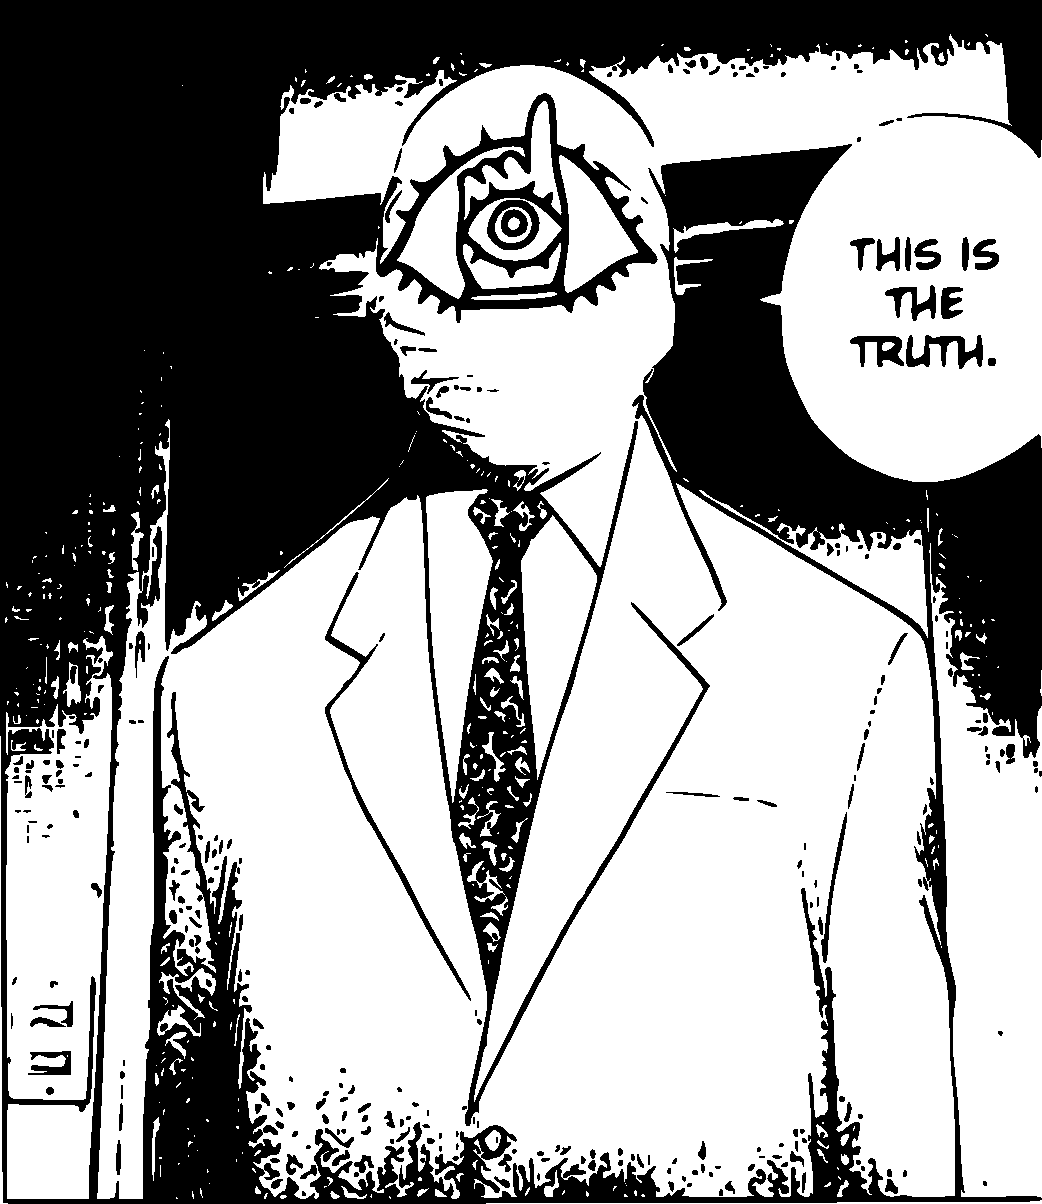
\includegraphics[width=0.4\textwidth,right ]{../../preamble/tomodachi.pdf} 
\end{figure}
\newpage %\setmainfont{Times New Roman}
\normalsize

\tableofcontents 
\newpage

%==================FOOTER e HEADER=======================%
\fancyhf{}
\fancyhead[L]{\nouppercase{\leftmark}}
\fancyhead[R]{Sezione \thesection}
\fancyfoot[C]{\thepage}
\fancyfoot[L]{\titolo}
\fancyfoot[R]{ Marco Casu}
%\fancyfoot[R]{\setmainfont{Palace Script MT}\huge Marco Casu \setmainfont{Times New Roman}}
%==================FOOTER e HEADER=======================%
\newtheorem{definition}{Definition}
\newtheorem{proposition}{Proposition}
%==================INIZIO======================%
\chapter{Introduction}
In this chapter we will see a brief introduction to the mathematical tools used in the main topics of the course. The topics presented in this section may seem somewhat unclear, as many concepts and definitions are only briefly introduced and deliberately not elaborated upon. They will be discussed in detail in their respective chapters.\bigskip
\section{About the End Effector Pose}
A robot is made up of a series of arms connected to one another by joints, these joints can be \textbf{revolut} or \textbf{prismatic} (as shown in figure \ref{img:joints}), a revolut joint rotate the link connected along 1 axis, the prismatic joint can make the link extend or contract, making them translate along 1 axis.

\begin{figure}[h!]
    \centering
    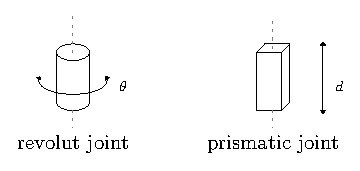
\includegraphics[width=0.6\textwidth ]{images/joints.eps} 
    \caption{two types of joints (spatial representation)}
    \label{img:joints}
\end{figure}

It is important to know that that if the angle $\theta$ increase the joint is rotating counter clock wise. In a planar drawing, the joints are denoted as shown in image \ref{img:joints_planar}.

\begin{figure}[h!]
    \centering
    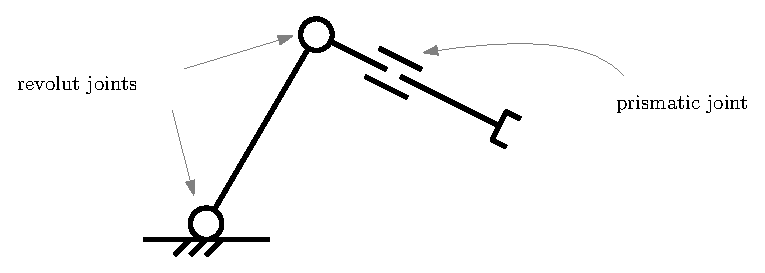
\includegraphics[width=0.6\textwidth ]{images/joints_planar.eps} 
    \caption{planar representation of the joints}
    \label{img:joints_planar}
\end{figure}

In the mathematical/geometrical model of a robotic arms, it is important the \textit{kinematic skeleton}, the quantities involved are\begin{itemize}
    \item the current angle of the joints
    \item the length of the links
\end{itemize}
everything is defined respect to the base frame, usually denoted as $\Sigma_0$.

\begin{figure}[h!]
    \centering
    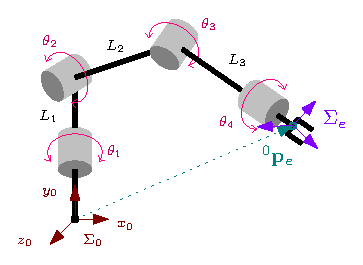
\includegraphics[width=0.45\textwidth ]{images/spatial_robot_new.eps} 
    \caption{spatial R4 robot}
    \label{img:spatialR4}
\end{figure}
\bigskip

The robot shown in figure \ref{img:spatialR4} is an \textit{R4 robot} (4 revolut joints) with three links. With ${}^0\mathbf p_e$ and $\Sigma_e$ we denote the position and the reference frame of the \textbf{end effector}, if there are a 0 supscript to a vector, we mean that is expressed in the base reference frame.\bigskip

With \textbf{Direct Kinematics}, we define the problem to find what are the \textbf{pose} (position and orientation) of the end effector, in function of the joint's angles. \begin{align}
    &Kin_p(\boldsymbol{\theta}):\Sigma_0\rightarrow\Sigma_e\\
    &\boldsymbol{\theta}=\begin{pmatrix}
        \theta_1&\theta_2&\theta_3&\theta_4
    \end{pmatrix}^T
\end{align}
With $\Sigma_e$ is denoted the reference frame of the end effector. How can we compute $Kin_p(\boldsymbol{\theta})$? This is given by an homogeneous $4\times 4$ matrix defined as follows:\begin{equation}
    {}^0T_e=\begin{pmatrix}
        & & & \\
        & {}^0R_e & &{}^0\mathbf p_e \\
        & & & \\
        0& 0&0 &1 
    \end{pmatrix}
\end{equation}
where\begin{itemize}
    \item ${}^0R_e\in SO(3)$ is the rotation matrix, and depends from $\boldsymbol{\theta}$
    \item ${}^0\mathbf p_e\in \R^3$ is the translation vector.
\end{itemize}

\noindent\textbf{Recall}: $SO(3)$ is the group of all the orthogonal $3\times 3$ matrices with determinant equals to 1.\bigskip

\noindent The matrix ${}^0T_e$ is obtained by multiplying $n$ matrix (where $n$ is the number of joints)\begin{align}
     &{}^0T_e= {}^0A_1(\theta_1) {}^1A_2(\theta_2)\dots {}^{n-1}A_n(\theta_n)=\\&\prod_{i=0}^{n-1}{}^iA_{i+1}(\theta_{i+1}).
\end{align}
Each \textit{homogeneous matrix} $^{i-1}A_i$ describe the pose of the $i$-th joint's frame respect to the previous joint's frame, and depends from $\theta_i$ (the $i$-th joint's angle). A more detailed description of the matrix describing the direct kinematics will be given later.\bigskip


If there are another frame $\Sigma_w$, the new matrix can be computed as follows\begin{equation}
    {}^w T_e={}^w T_0{}^0 T_e.
\end{equation}\begin{center}
    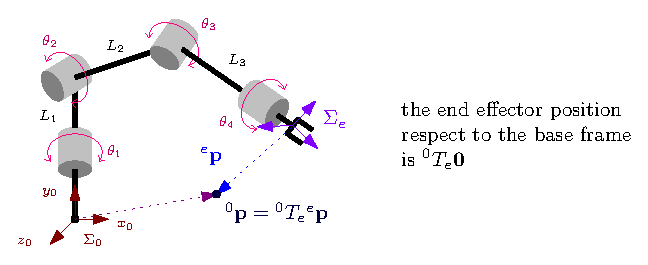
\includegraphics[width=0.8\textwidth ]{images/T_matrix_new.eps} 
\end{center}

The \textbf{Inverse Kinematics} is the opposite problem, given a position ${}^0\mathbf p_e$ for the end effector, we want to find the values of $\boldsymbol\theta$ such that\begin{equation}
    {}^0\mathbf p_e=Kin_p(\btheta)
\end{equation}
to find $\btheta$, we have to solve a non-linear system of equations, this is generally an undecidable problem, but for some specific cases, there exists a closed form, that can be found analytically, there are also numerical methods. Clearly, for the positions out of the work space, the system does not admit solutions (also this can be checked analytically).
\section{About the End Effector Velocity}
Let's now consider \textbf{Differential Kinematics}, that is the problem to find the end effector velocity in the workspace given the velocity of the joint's angles. 
Since the superposition principle is valid, the components resulting from the movement of each individual joint, which constitute the final velocity of the end effector, can be considered separately. It is important to know that the velocity component of the end effector given by a joint, is always orthogonal to the rotation axis of that joint.\bigskip

\noindent The end effector have\begin{itemize}
    \item a linear velocity, usually denoted $\mathbf v$
    \item an angular velocity, usually denoted $\bomega$.
\end{itemize}
\begin{figure}[h!]
    \centering
    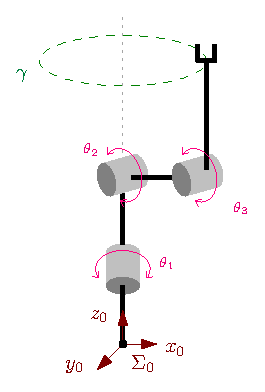
\includegraphics[width=0.28\textwidth ]{images/velocity_new.eps} 
    \caption{possible trajectory by moving $\theta_1$}
    \label{img:velocity_trajectory}
\end{figure}

In the figure \ref{img:velocity_trajectory} the curve $\gamma$ represent all possible positions where the end effector could lie if the angle $\theta_1$ change, the linear velocity of the end effector is orthogonal to the $z_0$ axis. The velocity of the end effector doesn't depend only from the angular velocity, but also from the current configuration of the angles $\btheta$.\bigskip

Even if the end effector is a rigid body, is sufficient to know the linear velocity of only one point and his angular velocity to compute the velocity of all the other points, since the following relation holds:\begin{equation}
    \mathbf v_2 = \mathbf v_1+\bomega\times \mathbf r_{12}
\end{equation}
where\begin{itemize}
    \item $\mathbf v_1$ is the velocity of the first point
    \item $\mathbf v_2$ is the velocity of the second point
    \item $\bomega$ is the angular velocity of the rigid body
    \item $\mathbf r_{12}$ is the difference between the positions of the two points.
\end{itemize}
Let's analyze the velocity components of the end effector. If the $i$-th joint is changing is angle, the linear velocity of the end effector will have one component that is\begin{equation}
    \mathbf v_i=\mathbf j_i(\btheta)\dot\theta_i
\end{equation}
where $\mathbf j_i$ is a 3 components vector describing the direction of the velocity.
Since the direction depends from the configuration, the vector $\mathbf j_i$ is in function of $\btheta$.
This holds for all the angles $\theta_i$, the resultant linear velocity of the end effector will be\begin{equation}
    \mathbf v=\sum_{i=1}^n\mathbf j_i(\btheta)\dot\theta_i
\end{equation}
it can be written in matrix form\begin{equation}
    \mathbf v = J_L(\btheta)\dot\btheta=\begin{pmatrix}
        &&\\
        \mathbf j_1(\btheta)&\dots&\mathbf j_n(\btheta)\\
        &&
    \end{pmatrix}\begin{pmatrix}
        \dot\theta_1\\\dot\theta_2\\\dot\theta_3
    \end{pmatrix}
\end{equation}
where $J_L(\btheta)$ is a $3\times n$ matrix called the \textbf{Jacobian Matrix}, where $n$ is the number of joints. This description were given in terms of the linear velocity, but it holds also for the angular velocity of the end effector, indeed we have two Jacobian Matrix:\begin{itemize}
    \item we denote $J_L(\btheta)$ the Jacobian matrix for the linear velocity
    \item we denote $J_A(\btheta)$ the Jacobian matrix for the angular velocity\begin{equation}
        \bomega=J_A(\btheta)\dot\btheta
    \end{equation}
\end{itemize}
the matrix\begin{equation}
    J(\btheta)=\begin{pmatrix}
        J_L(\btheta)\\
        J_A(\btheta)
    \end{pmatrix}\in Mat(6\times n)
\end{equation}
it's called \textbf{basic Jacobian}.\bigskip

The Jacobian matrix is a mapping from the joint velocity space to the end effector velocity space. Let's ignore the angular velocity for now, suppose that we want to impose to the end effector a desired linear velocity (in a specific time instant)\begin{equation}
    \mathbf v=\mathbf v_d\in\R^3
\end{equation}
we need to find the values for the vector $\dot\btheta$ such that \begin{equation}\label{eq:diff_inv_kin}
    \mathbf v_d=J_L(\btheta)\dot\btheta
\end{equation}
if we have 3 joints, the matrix $J$ is squared and can be inverted\begin{equation}
    \dot\btheta=J_L^{-1}(\btheta) \mathbf v_d
\end{equation}
but this is not the general case, if $n>3$, the system of equations given in \eqref{eq:diff_inv_kin} could\begin{itemize}
    \item have zero solutions
    \item have infinite solutions
\end{itemize}
if the determinant of $J_L^{-1}$ is zero, the system admit infinite solutions if and only if the desired velocity vector $\mathbf v_d$ is in the range space of $J_L^{-1}$\begin{equation}
    \det J_L^{-1}=0\implies \exists \text{ inf. sol. }\iff   \mathbf v_d\in \text{Range}(J_L^{-1})
\end{equation}
we remind that the range space of a matrix, is the set of all the linear combinations of the matrix's columns. If this isn't true, the system does not admit any solution, it means that no possible combination of velocity $\dot\btheta$ could realize the desired end effector velocity. 
\subsection{Singularity}
Let's talk about \textbf{singularities} in the joint velocity space, we will give a geometric example. Let's consider a 2R planar robot, with a fixed joints configuration $\btheta$, the Jacobian is a $2\times 2$ matrix. Let $\mathbf v_d$ to be the desired velocity, the system is the following\begin{equation}
    \begin{pmatrix}
        v_d^x\\v_d^y
    \end{pmatrix}=
    \begin{pmatrix}
       \mathbf j_1^T\\\mathbf j_2^T
    \end{pmatrix}
    \begin{pmatrix}
        \dot\theta_1\\\dot\theta_2
    \end{pmatrix}
\end{equation}
the two linear equation of the system is represented on the plane as two lines. If $\det J_L\ne 0$, there are only one solution, and is the intersection between the two lines.
\begin{center}
    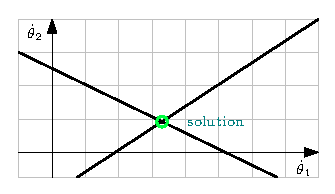
\includegraphics[width=0.4\textwidth ]{images/system_one_sol.eps} 
\end{center}
If $\det J_L= 0$, the two lines are parallel, so either they have no intersection, or they are the same line. If there are infinite solutions, we can choose the one with the smallest norm, since represents the ''minimum energy'' solution (the solution that requires the least joint rotation speed intensity).
\begin{center}
    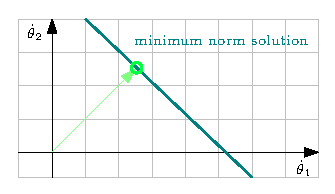
\includegraphics[width=0.4\textwidth ]{images/infinite_sol.eps} 
\end{center}
We have a \textit{singularity} when the determinant approaches zero\begin{equation}
    \det J_L\rightarrow 0
\end{equation}
The closer the determinant (in absolute value) gets to zero, the more "nearly" parallel the row vectors (and thus the lines they represent) become, which means the angle of intersection approaches zero. In this case the norm of the solution could be large.
\begin{center}
    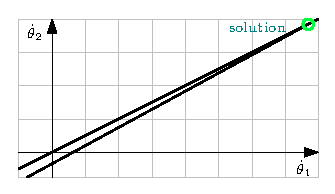
\includegraphics[width=0.4\textwidth ]{images/singularity.eps} 
\end{center}
This is true also because the following relations holds
\begin{align}
    &J_L=\begin{pmatrix}
        j_{11}&j_{12}\\
         j_{21}&j_{22}
    \end{pmatrix}\implies\\ &J_L^{-1}=\frac{1}{\det J_L}\begin{pmatrix}
        j_{22}&-j_{12}\\
         -j_{21}&j_{11}
    \end{pmatrix}\\
    &\mathbf v_d=J_L\dot\btheta\\
    &\dot\btheta=J_L^{-1}\mathbf v_d\\
      &\dot\btheta=\frac{1}{\det J_L}\begin{pmatrix}
        j_{22}&-j_{12}\\
         -j_{21}&j_{11}
    \end{pmatrix}\mathbf v_d
\end{align}
with $\det J_L\rightarrow 0$ the term $\frac{1}{\det J_L}$ (and with it, also $\dot\btheta$) became bigger and bigger. In this case, the required joint rotation velocity might not be achievable by the robotic arm's motors.\bigskip

The previous example showed how certain algebraic relationships are connected to physical problems in robot joint control. Another similar example is the following, consider the robotic arm shown in figure \ref{img:impossible_traj}.

\begin{figure}[h!]
    \centering
    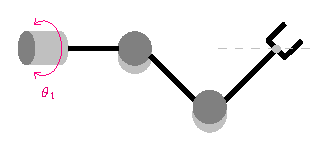
\includegraphics[width=0.4\textwidth ]{images/impossible_velocity_new.eps} 
    \caption{3R spatial robot}
    \label{img:impossible_traj}
\end{figure}

Geometrically, it can be seen that by rotating only the first joint $\theta_1$, the position of the end effector will not change, this condition holds when\begin{equation}
    J_L(\btheta)\begin{pmatrix}
        \dot\theta_1\\0\\0
    \end{pmatrix}=\begin{pmatrix}
        0\\0\\0
    \end{pmatrix}
\end{equation}
this is true if the vector $\begin{pmatrix}
        \dot\theta_1&0&0
    \end{pmatrix}^T$ is in the kernel of the Jacobian matrix\begin{equation}
        \begin{pmatrix}
        \dot\theta_1\\0\\0
    \end{pmatrix}\in \ker J_L(\btheta).
    \end{equation}

Therefore, the vectors contained in the kernel of the Jacobian matrix for the linear (or angular) velocity represent all possible combinations of individual joint velocities that would not change the position (or orientation) of the end effector.
\section{Brief Overview of Planning and Control}
When we want to control the end effector of a robotic arm, we want to know how to move the joints to get a specific position for the end effector, and also how to control the joints over the time to get a particular \textit{trajectory} in the working space. 

Consider a 2R planar robot, as shown in figure \ref{img:2R_planar}, where $\btheta$ is the angular position of the joints, and $\mathbf p_e=f(\btheta)$ is the position of the end effector for some $f_\R^2\rightarrow\R^2$.\bigskip

\begin{figure}[h!]
    \centering
    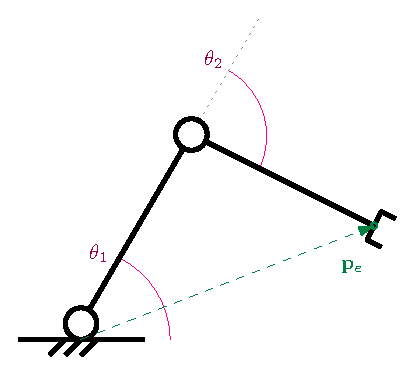
\includegraphics[width=0.5\textwidth ]{images/2R_planar.eps} 
    \caption{a 2R planar robot}
    \label{img:2R_planar}
\end{figure}

We would like to move the end effector from a certain starting point $\mathbf p_a\in \R^2$ to an another point $\mathbf p_b\in\R^2$. We could consider the segment line from $\mathbf p_a$ to $\mathbf p_b$ defined as follows:\begin{equation}
    \mathbf p(s)=s\mathbf p_b+(1-s)\mathbf p_a \ \ \ \ \ s\in[0,1].
\end{equation}
Such a trajectory can be represented by a time-dependent function that starts from an initial time $t_0=0$ until a final time $T$, making $s$ a monotonically increasing function of $t\in[0,T]$:\begin{align}
    &s:[0,1]\longmapsto [0,T]\\
    &s(0)=0\\
    &s(1)=T\\
    &\mathbf p(s)=\mathbf p(s(t))
\end{align}
We say that a trajectory is rest-to-rest if the velocity of the end effector at the start and at the end of that trajectory is zero:\begin{equation}
    \dot{\mathbf p}(s(0))=\dot{\mathbf p}(s(T))=\mathbf 0
\end{equation}
 we need to include boundary conditions. Considering the chain rule, the derivative of $\mathbf p$ respect to the time $t$ is\begin{equation}
    \dot{\mathbf p}=\frac{d\mathbf p}{dt}=\frac{d\mathbf p}{ds}\frac{ds}{dt}=\frac{d\mathbf p}{ds}\dot s
\end{equation}
since\begin{equation}
    \frac{d\mathbf p}{ds}=\frac{d}{ds}\left(s\mathbf p_b+(1-s)\mathbf p_a\right)=\mathbf p_b-\mathbf p_a
\end{equation}
we have
\begin{equation}
    \dot{\mathbf p}=\frac{d\mathbf p}{ds}\dot s=\dot s(\mathbf p_b-\mathbf p_a)
\end{equation}
the acceleration is\begin{equation}
    \ddot{\mathbf p}=\ddot s(\mathbf p_b-\mathbf p_a)+\dot s\cdot \mathbf 0=\ddot s(\mathbf p_b-\mathbf p_a)
\end{equation}
we have that\begin{align}
    &\dot{\mathbf p}(s(0))=0\iff \dot s(0)(\mathbf p_b-\mathbf p_a)\iff \dot s(0)=0\\
    &\dot{\mathbf p}(s(T))=0\iff \dot s(T)(\mathbf p_b-\mathbf p_a)\iff \dot s(T)=0
\end{align}
The starting velocity and the final velocity is zero, so the variation of the velocity is zero, this can be seen by the integral of the acceleration\begin{equation}
    \int_0^T\ddot{\mathbf p}dt=\int_0^T\ddot s(\mathbf p_b-\mathbf p_a)dt=(\mathbf p_b-\mathbf p_a)\int_0^T\ddot sdt=(\mathbf p_b-\mathbf p_a)(\dot s(T)-\dot s(0))=0.
\end{equation}
Let's see an example, let's say that the linear position of the end effector along 1 axis is given by the law\begin{equation}
    s(t)
\end{equation}\begin{center}
    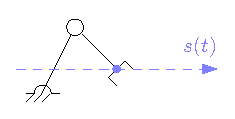
\includegraphics[width=0.5\textwidth ]{images/lin_pos.eps} 
\end{center}
we have the following profile for the acceleration:
\begin{equation}
    \ddot s(t)=\begin{cases}
        1\text{ if }t\in[0,1]\cup [\frac{3}{8},4]\cup [\frac{5}{8},\frac{7}{8}]\\
        -1\text{ if }t\in[1,\frac{3}{8}]\cup [4,\frac{5}{8}]\cup [\frac{7}{8},8]
    \end{cases}
\end{equation}
Let's assume that\begin{equation}
    \dot s(0)=s(0)=0
\end{equation}
\begin{itemize}
    \item Question: What will be the speed of the end effector at $t=8$? We can easily see that the integral of $\ddot s$ over $t\in [0,8]$ is 0, so $\Delta\dot s =0\implies \dot s(8)=0$.
    \item Question: What will be the position of the end effector at $t=8$? We can easily see that the integral of $\dot s$ over $t\in [0,8]$ is 0, so $\Delta s =0\implies  s(8)=0$.
\end{itemize}
The acceleration, speed and position profiles are the following:\begin{center}
    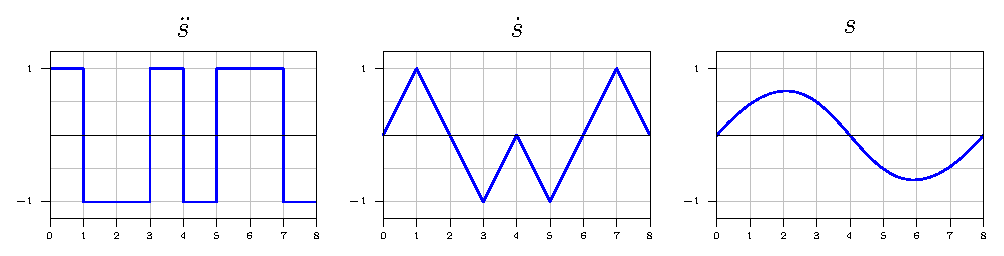
\includegraphics[width=1\textwidth ]{images/profiles.eps} 
\end{center}
Now we consider the \textit{control aspects} of the problem, we denote $\mathbf p_e(t)$ the position of the end effector at the time $t$, and $\mathbf p_d(t)$ the \textbf{desired position} at time $t$.\begin{equation}
    \mathbf p_d(0)=\mathbf p_a.
\end{equation}
We define the \textbf{error} such as the difference between the current position and the desired position:\begin{eqnarray}
    \mathbf e(t)=\mathbf p_d(t)-\mathbf p_e(t)
\end{eqnarray}
The aim of the \textit{control system} of the robot is to maintain $\mathbf e$ as close to zero as possible. This can be done by computing the initial error, and by giving to the system a new command $\dot\btheta(t)$ to correct it such that $\mathbf e(t)\rightarrow\mathbf 0$. Let's denotate the error as follows\begin{equation}
    \mathbf e(t)=\begin{pmatrix}
        e_x(t)\\ e_y(t)
    \end{pmatrix}
\end{equation}
For now, we will not discuss in detail how to control the error through the control of joint velocities $\dot\btheta$; it is sufficient to know that the following condition is required:\begin{equation}
    \dot{\mathbf e}(t)=-K\mathbf e(t)=\begin{pmatrix}
        -k_x&0\\
        0&-k_y
    \end{pmatrix}\begin{pmatrix}
        e_x(t)\\ e_y(t)
    \end{pmatrix}
\end{equation}
with $k_x,k_y>0$.
Why this conditions is required?\begin{itemize}
    \item if $e_x(t)$ is greater than zero, the condition $\dot e_x(t)=-k_xe_x(t)$ describes a decrease in error, making it approach zero 
    \item if $e_x(t)$ is smaller than zero, the condition $\dot e_x(t)=-k_xe_x(t)$ describes an increase in error, making it approach zero 
    \item same for $e_y$.
\end{itemize}
The system of equations\begin{equation}
    \dot{\mathbf e}(t)=\begin{pmatrix}
        -k_x&0\\
        0&-k_y
    \end{pmatrix}\begin{pmatrix}
        e_x(t)\\ e_y(t)
    \end{pmatrix}\implies \begin{cases}
        \dot e_x(t)=-k_xe_x(t)\\
        \dot e_y(t)=-k_ye_y(t)
    \end{cases}
\end{equation}
admits exponential functions as a solution\begin{align}
    &e_x(t)=e_x(0)e^{-k_xt}\\
    &e_y(t)=e_y(0)e^{-k_yt}
\end{align}
if the initial error $\mathbf e(0)$ is not zero, then the error will approaches zero, without never reaching it. For practical applications it goes sufficiently
fast to values very close to zero.\bigskip

\noindent We introduce now an important concept in linear differential equations systems.\begin{definition}
    Let $A\in M_{n,n}(\R)$ to be a squared real-valued matrix. The \textbf{matrix exponential}, denoted $e^A$, is the $n\times n$ matrix defined as follows:\begin{equation}
        e^A=\sum_{k=0}^\infty\frac{A^k}{k!}
    \end{equation}
\end{definition}
Given a linear system\begin{equation}
    \dot{\mathbf x}=A\mathbf x
\end{equation}
the solution is\begin{equation}
    \mathbf x(t)=e^{At}\mathbf x(0)
\end{equation}
In some cases the exponential matrix can be computed easily, let's assume that $A$ is diagonal\begin{equation}
    A=\begin{pmatrix}
a_1 & 0 & \cdots & 0 \\
0 & a_2 & \cdots & 0 \\
\vdots & \vdots & \ddots & \vdots \\
0 & 0 & \cdots & a_n
\end{pmatrix}
\end{equation}
in this case we have that\begin{equation}
    A^k=\begin{pmatrix}
a_1 & 0 & \cdots & 0 \\
0 & a_2 & \cdots & 0 \\
\vdots & \vdots & \ddots & \vdots \\
0 & 0 & \cdots & a_n
\end{pmatrix}\times  \dots \times \begin{pmatrix}
a_1 & 0 & \cdots & 0 \\
0 & a_2 & \cdots & 0 \\
\vdots & \vdots & \ddots & \vdots \\
0 & 0 & \cdots & a_n
\end{pmatrix} = \begin{pmatrix}
a_1^k & 0 & \cdots & 0 \\
0 & a_2^k & \cdots & 0 \\
\vdots & \vdots & \ddots & \vdots \\
0 & 0 & \cdots & a_n^k
\end{pmatrix}
\end{equation}
so\begin{align}
    &e^A=\sum_{k=0}^\infty\frac{1}{k!}\begin{pmatrix}
a_1^k & 0 & \cdots & 0 \\
0 & a_2^k & \cdots & 0 \\
\vdots & \vdots & \ddots & \vdots \\
0 & 0 & \cdots & a_n^k
\end{pmatrix}=
\begin{pmatrix}
\sum_{k=0}^\infty\frac{a_1^k}{k!} & 0 & \cdots & 0 \\
0 & \sum_{k=0}^\infty\frac{a_2^k}{k!} & \cdots & 0 \\
\vdots & \vdots & \ddots & \vdots \\
0 & 0 & \cdots & \sum_{k=0}^\infty\frac{a_n^k}{k!}
\end{pmatrix}\\& =
\begin{pmatrix}
e^{a_1} & 0 & \cdots & 0 \\
0 & e^{a_2} & \cdots & 0 \\
\vdots & \vdots & \ddots & \vdots \\
0 & 0 & \cdots & e^{a_n}
\end{pmatrix}.
\end{align}
So, if a system is described by a diagonalizable matrix $A$ there exists a diagonal matrix 
$\Lambda$ and an invertible matrix $T$ such that\begin{equation}
    A=T\Lambda T^{-1}
\end{equation}
in this case we can easily calculate the exponential matrix\begin{equation}
    e^{At}=T^{-1}e^{\Lambda t} T.
\end{equation}

\noindent\textbf{Note}: The Sections  \ref{gemini:def}, \ref{gemini:ethical}, \ref{gemini:ev}, \ref{gemini:examples}, \ref{gemini:statistics} are written with the aid of Gemini, by having the model process the information taken from the professor's slides and the lecture notes.

\section{Defining Robots}\label{gemini:def}
The concept of a robot is formalized through several key definitions, spanning from strict industrial standards to more encompassing theoretical perspectives.

\subsection{Standardized Definitions}

\subsubsection*{1. Industrial Definition (Robotic Institute of America - RIA)}
The RIA defines a robot as a \textbf{re-programmable, multi-functional manipulator} designed to move material, parts, tools, or specialized devices through variable programmed motions for the performance of a variety of tasks. A crucial element of this definition is the requirement that the robot must \textbf{acquire information from the environment} and move intelligently in response, setting it apart from simpler automated machinery.

\subsubsection*{2. ISO 8373:2012 Definition}
The International Organization for Standardization (ISO) provides a formal, international standard: an industrial robot is an \textbf{automatically controlled, re-programmable, multi-purpose manipulator} programmable in \textbf{three or more axes}. The manipulator may be either \textbf{fixed in place or mobile} and is intended for use in industrial automation applications. This specific definition helps to delineate complex, versatile machines from basic mechanical devices.

\subsection{The Visionary Definition: Perception and Action}
A broader, more "visionary" definition emphasizes the cognitive and functional aspects of robotic systems: the \textbf{intelligent connection between perception and action}.

\begin{itemize}
    \item \textbf{Perception:} This is the process of acquiring and processing sensing information from the environment.
    \item \textbf{Action:} This involves not just controlling the robot's current state, but actively \textbf{making some changes in the physical world} to achieve a goal.
\end{itemize}

This relationship forms a continuous feedback loop that governs autonomous behavior:
$$\text{percept} \longrightarrow \text{action} \longrightarrow \text{percept}$$
The robot's understanding of its environment (\textit{percept}) drives its movement or operation (\textit{action}), which modifies the environment, leading to a new cycle of perception.

\section{Notable Robot Examples}\label{gemini:examples}
Throughout history, various robots have exemplified different facets of the definition of robotics, from pure industrial work to exploration and human interaction.

\begin{itemize}
    \item \textbf{Comau H4 (1995):} Representing the industrial segment, these manipulators were widely used in \textbf{automotive industries} (e.g., owned by Fiat at the time). They are a classic example of fixed, multi-functional, re-programmable automation.
    
    \item \textbf{Waseda WAM-8 (1984):} This famous \textbf{humanoid robot} from a Japanese university demonstrated early cognitive abilities. It was capable of complex tasks such as playing an organ and reading music from a sheet, combining perception (reading) and fine manipulation.
    
    \item \textbf{Spirit Rover (2002):} An excellent example of \textbf{autonomous mobile robotics and exploration}.
    \begin{itemize}
        \item It was landed on Mars, featuring articulated wheels and solar panels.
        \item Its mission was to move, analyze material, and send gathered information back to Earth.
        \item While the \textbf{global target} is \textbf{specified remotely}, the rover must operate with significant \textbf{local autonomy} because of the approximately 8-minute communication delay required to receive instructions from Earth. This necessity highlights the critical role of the onboard perception-action loop for mission success.
    \end{itemize}
\end{itemize}
\begin{figure}[h!]
    \centering
    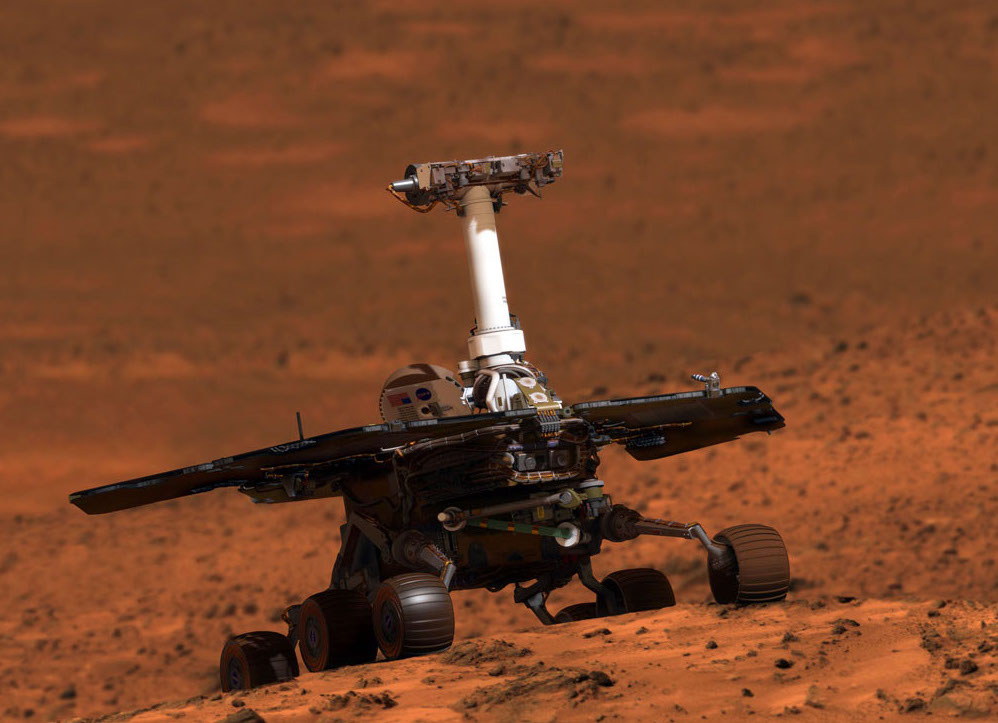
\includegraphics[width=0.4\textwidth ]{images/rover.jpg} 
    \caption{Spirit Rover (2002)}
\end{figure}

According to the rigorous \textbf{ISO 8373:2012} definition, certain devices and systems are \textbf{not considered robots}. These exclusions are typically applied to specific devices with only \textbf{one or two degrees of freedom (DOF)} and complex software systems lacking the physical manipulator required by the standard.
Systems that are not classified as robots under the ISO 2012 standard include:
\begin{itemize}
    \item Software ''bots'', Artificial Intelligence (AI), and Robotic Process Automation (RPA).
    \item Voice assistants.
    \item Automatic Teller Machines (ATMs).
    \item Cooking machines, smart washing machines, and similar appliances.
\end{itemize}
Furthermore, advanced mobile systems like drones and autonomous cars are generally not classified as robots under this definition. However, in a \textbf{2021 revision}, the term \textbf{robotic device} was introduced to encompass these increasingly sophisticated, automated machines that fall outside the strict definition of an industrial robot.\bigskip


The word ''robot'' has an historical and literary origin that is foundational to the field:
\begin{itemize}
    \item The term derives from the Slavic word \textbf{Robota}, meaning ''work'' or ''forced labor.''
    \item The first recorded use of the word ''Robot'' in a theatrical context was in \textbf{1920} by Czech writer \textbf{Karel Čapek} in his science-fiction play, \textit{Rossum's Universal Robots (R.U.R.)}. In the play, ''robots'' are artificial, human-like creatures created to be inexpensive workers.
\end{itemize}

\section{The Ethical Framework: Asimov's Three Laws of Robotics}\label{gemini:ethical}
The science fiction author Isaac Asimov defined a set of foundational ethical rules for robotics in his short stories.

\begin{enumerate}
    \item \textbf{First Law:} A robot may not injure a human being or, through inaction, allow a human being to come to harm.
    \begin{itemize}
        \item This law is fundamental to modern \textbf{collaborative robotics} (cobots), ensuring human safety is prioritized as robots and humans work in close proximity.
    \end{itemize}
    \item \textbf{Second Law:} A robot must obey orders given to it by human beings, except where such orders would conflict with the First Law.
    \begin{itemize}
        \item This establishes the robot's subordination to human command. Situations like robots used in war or faulty programming clearly violate this rule.
    \end{itemize}
    \item \textbf{Third Law:} A robot must protect its own existence as long as such protection does not conflict with the First or Second Law.
    \begin{itemize}
        \item The robot's self-preservation is conditional, being secondary to human safety and commands.
    \end{itemize}
\end{enumerate}

\section{Evolution and Characteristics of Robot Manipulators}\label{gemini:ev}

The journey toward the industrial robot began around the 1950s with the convergence of \textbf{Computerized Numerically Controlled (CNC) machines} and \textbf{mechanical telemanipulators}. This synthesis led to the development of the first \textbf{robot manipulators}, with the \textbf{Unimation PUMA (1970)} being a key early example.\bigskip


Unlike the early mechanical telemanipulators, which often required continuous human control, true robot manipulators offered several distinct advantages:
\begin{itemize}
    \item \textbf{Absence of Position Memory:} The robot operates based on its programmed coordinates, not needing to remember past states.
    \item \textbf{Adaptivity} to conditions previously unknown.
    \item High \textbf{Accuracy} in positioning.
    \item Superior \textbf{Repeatability} of operation (the ability to return consistently to a programmed point).
\end{itemize}
For an industrial manipulator, it is often noted that \textbf{repeatability} and \textbf{compliance} (adaptivity to variations) are more fundamental for task success than absolute accuracy.\bigskip

The history of industrial robotics is marked by key patented designs and technological firsts:
\textbf{The First Industrial Robot}
The very first industrial robot was installed at a General Motors plant in \textbf{1961}. It was developed by \textbf{George Devol and Joseph Engelberger} of Unimation.
\begin{itemize}
    \item \textbf{Kinematics:} This design featured a total of \textbf{6 Degrees of Freedom (DOF)}, comprising five revolute (rotational) joints and one prismatic (linear) joint. This combination was considered the optimal solution at the time to achieve \textbf{full control over the end effector's pose} (position and orientation).
\end{itemize}

\textbf{Key Successor Robot Manipulators}
Following the first installation, several robots introduced foundational innovations:
\begin{itemize}
    \item \textbf{ASEA IRB-6 (1973):} The first robot where all axes were driven by \textbf{electric motors} (all-electric drives), featuring 5 DOF.
    \item \textbf{Cincinnati Milacron T3 (1974):} Recognized as the first industrial robot to be controlled by a \textbf{micro-computer}.
    \item \textbf{Hirata AR-300 (1978):} Introduced the first \textbf{SCARA (Selective Compliance Assembly Robot Arm)} robot, which has a distinct cylindrical workspace, prioritizing speed and rigidity in the vertical axis.
    \item \textbf{Unimation PUMA 560 (1979):} Characterized by its 6 revolute joints, this was the first truly \textbf{'anthropomorphic'} robot, offering human-like dexterity.
\end{itemize}\bigskip

\begin{figure}[h!]
    \centering
    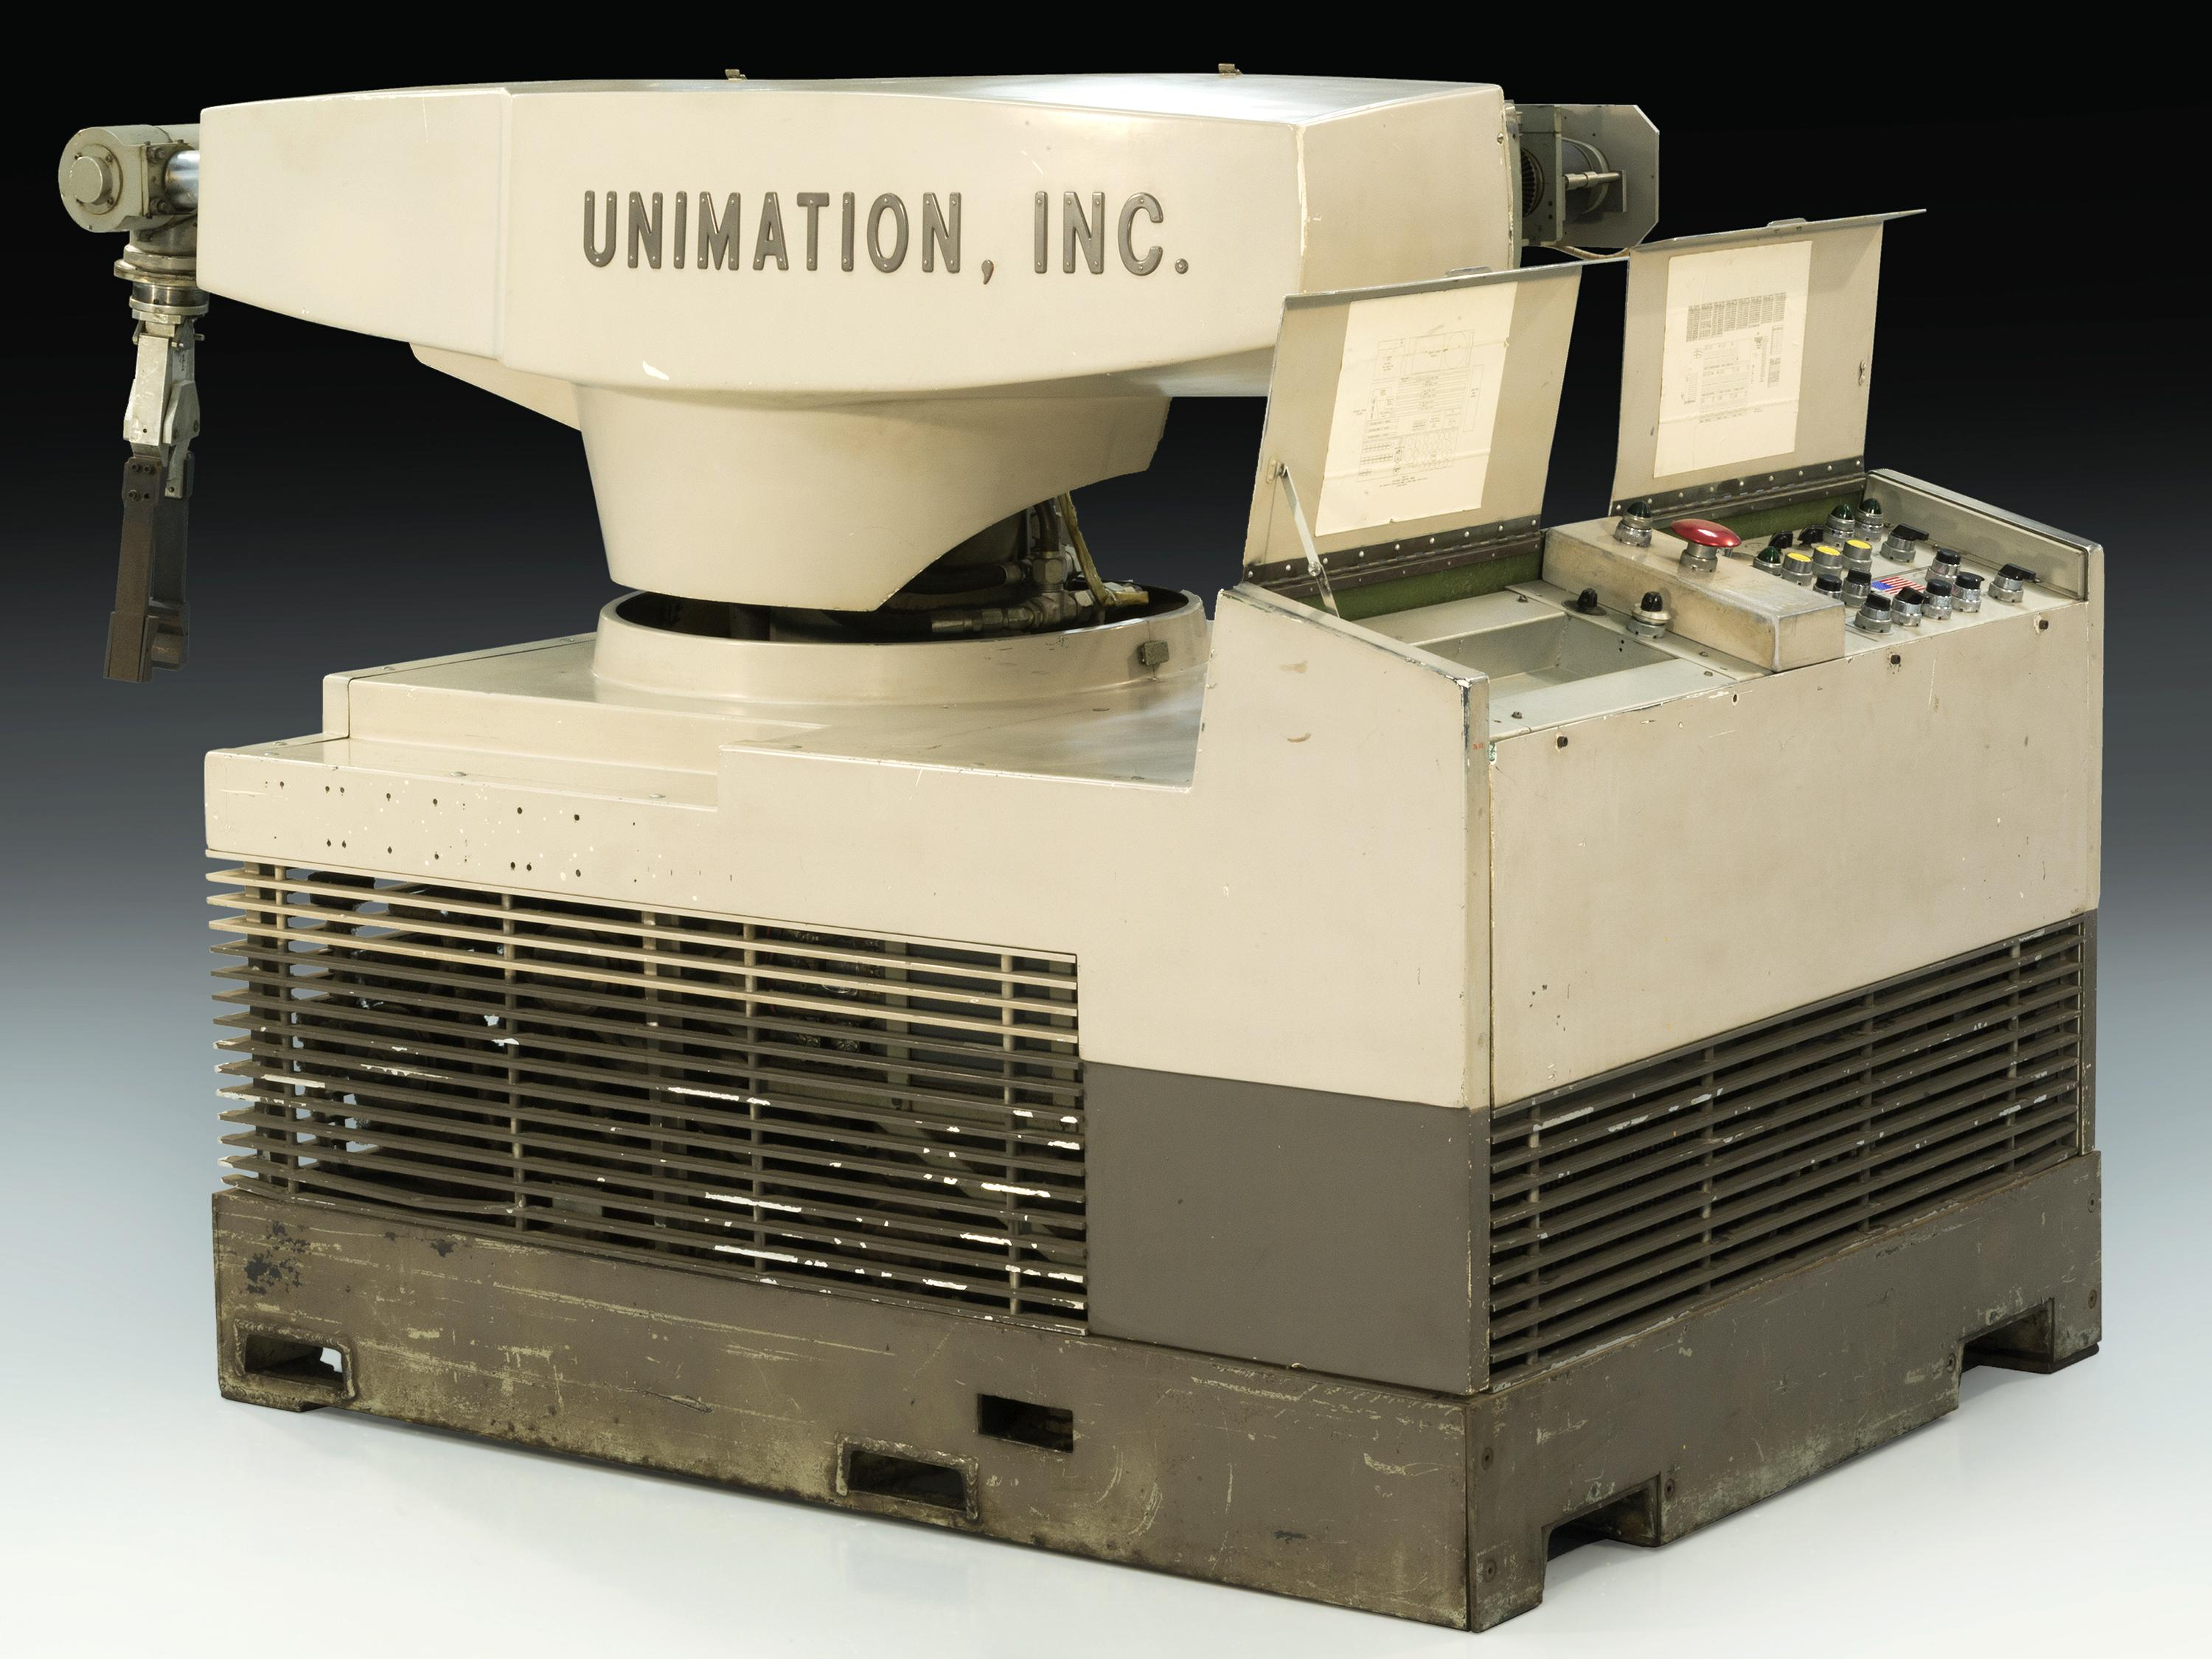
\includegraphics[width=0.4\textwidth ]{images/unimation.jpg} 
    \caption{Unimation PUMA 560 (1979)}
\end{figure}

Actuators power the robot and sustain its payload. \textbf{Electric motors} are the most common choice, converting electrical energy to torque. However, when required to sustain a \textbf{heavy payload}, a \textbf{hydraulic actuator} generally works better due to its higher power-to-weight ratio.
\section{Global Industrial Robotics Market Statistics}\label{gemini:statistics}

The following statistics are sourced from the \textbf{International Federation of Robotics (IFR)} World Robotics documents (Executive Summary for 2025 statistics). These figures illustrate the rapid global expansion of industrial automation.

\subsection{Operational Stock and Growth Rates}
The total worldwide operational stock of industrial robots reached \textbf{4.6 million units} at the end of 2024. This represents a substantial growth of \textbf{+9\%} compared to 2023. Over the five-year period from 2019 to 2024, the market demonstrated a robust Compound Annual Growth Rate (\textbf{CAGR}) of \textbf{+11\%}.

The Compound Annual Growth Rate is calculated as:
$$\text{CAGR} = \left(\frac{V_{\text{end}}}{V_{\text{begin}}}\right)^{1/\text{years}} - 1$$

New robot sales in 2024 reached \textbf{542,000 units}, maintaining stability ($\pm 0\%$) compared to 2023, and demonstrating a $+7\%$ CAGR from 2019–2024. This marks the \textbf{fourth consecutive year} that annual new installations have surpassed 500,000 units. The estimated average service life of an industrial robot is between \textbf{12 and 15 years}.

Regarding market size, the value of the robot market (excluding software and peripherals) was \textbf{\$15.7 billion} in 2022. The value of the total robotic systems market, which includes surrounding equipment and services, is estimated to be approximately \textbf{four times} this core market value.

\subsection{Sectoral and Geographic Distribution}
The market growth is primarily driven by the \textbf{electronics} and \textbf{automotive} industries, with collaborative robots (cobots) also contributing significantly to market expansion.

The global distribution of installations is highly concentrated:
\begin{itemize}
    \item \textbf{China} is the world's largest market for new installations, a position it has held since 2013. China installs \textbf{every other robot} globally, accounting for \textbf{54\%} of all new annual installations.
    \item A vast majority—\textbf{80\%} of all new robot installations—occur in just five countries: \textbf{China, Japan, USA, Korea, and Germany}.
    \item Within Europe, \textbf{Italy} stands out as the second-largest European country for new installations.
\end{itemize}

The scale of growth is highlighted by the historical operational stock data: starting from a modest 3,000 units in 1973, stock grew to 66K in 1983, 575K in 1993, and 800K in 2003, culminating in the 4.6 million units recorded in 2024.

\begin{figure}[h!]
    \centering
    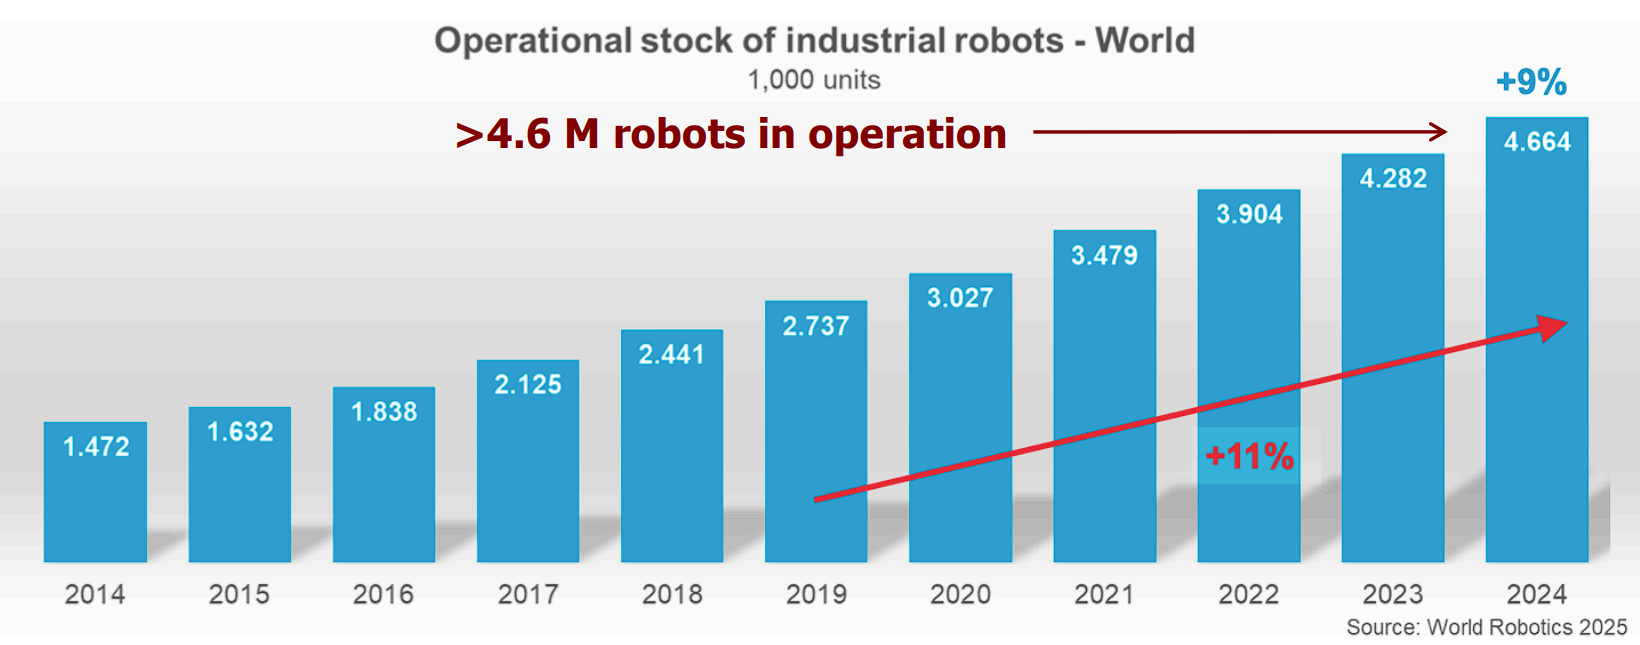
\includegraphics[width=0.9\textwidth ]{images/op_stocks.png} 
\end{figure}

\chapter{Sensors and Actuators}
From an high level prospective, a robot is a system composed by different units, that takes commands and responds with actions in a working environment, as shown in figure \ref{fig:system}.
\begin{figure}[h!]
    \centering
    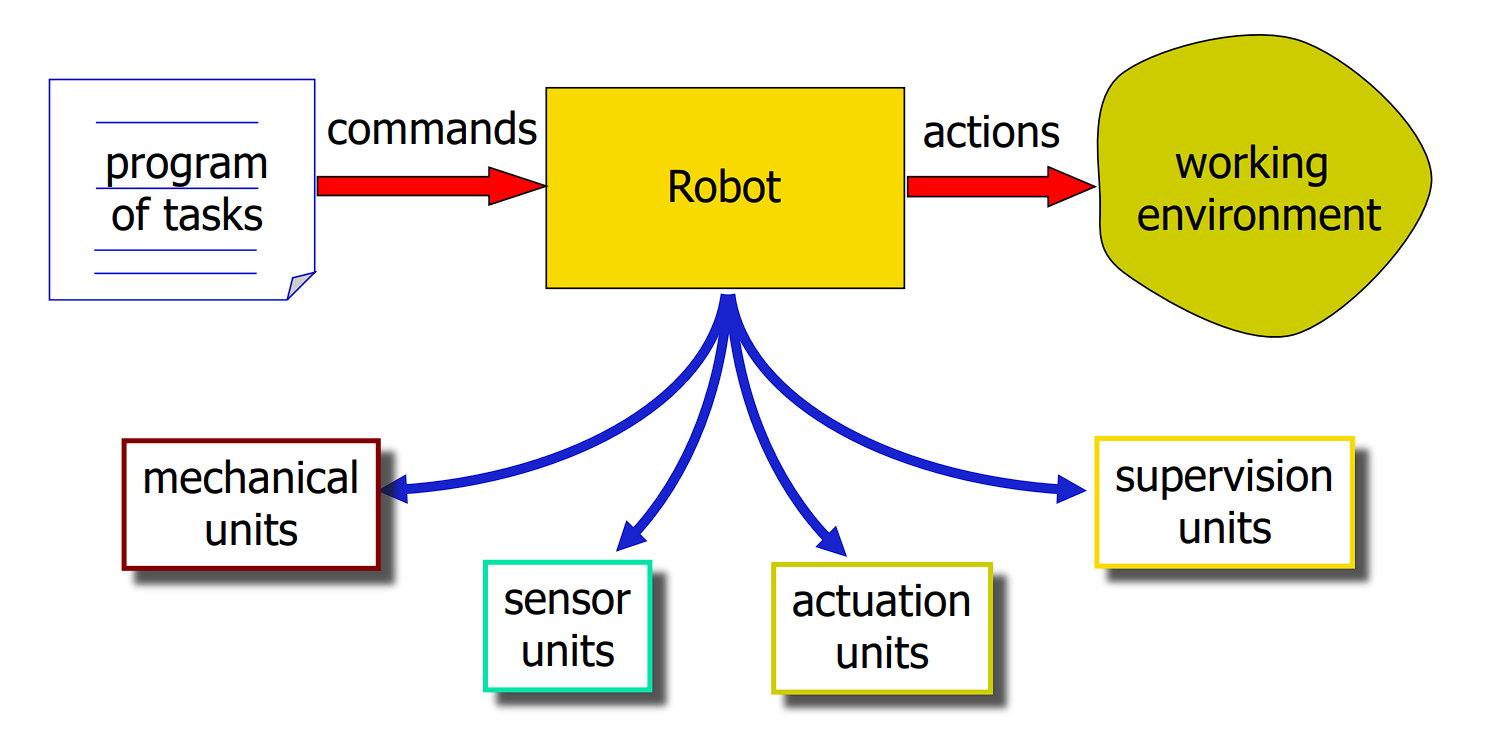
\includegraphics[width=0.7\textwidth ]{images/robosystem.png} 
    \caption{Robot as a system}
    \label{fig:system}
\end{figure}

The functional units are the following:\begin{itemize}
    \item mechanical units (robot arms): We see the links as rigid bodies, connected by rotational or prismatic joints, with an end effector attached at the end of the serial structure.
    \item actuation units: we have motors for the joints, that can be electrical, hydraulic or pneumatic, and eventually transmissions (i.g. a belt). We also consider the motion control algorithm as a part of that unit.
    \item sensor units: proprioceptive sensors that measure the internal state of the robot (position and velocity of the joints) and exteroceptive that measure the external environment.
    \item supervision units: AI and reasoning, task planning and control.
\end{itemize}
Let's focus on the actuation system, we can consider the scheme in figure \ref{fig:Actuationsystem}. We see how the power is measured in different units in different stage of the actuation process:\begin{itemize}
    \item Electrical : power = voltage $\times$ current
    \item Hydraulic : power = pressure $\times$ flow rate 
    \item Linear Mechanics : power = force $\times$ speed 
    \item Rotational Mechanics : power = torque $\times$ angular speed
\end{itemize}
{fig:system}.

\begin{figure}[h!]
    \centering
    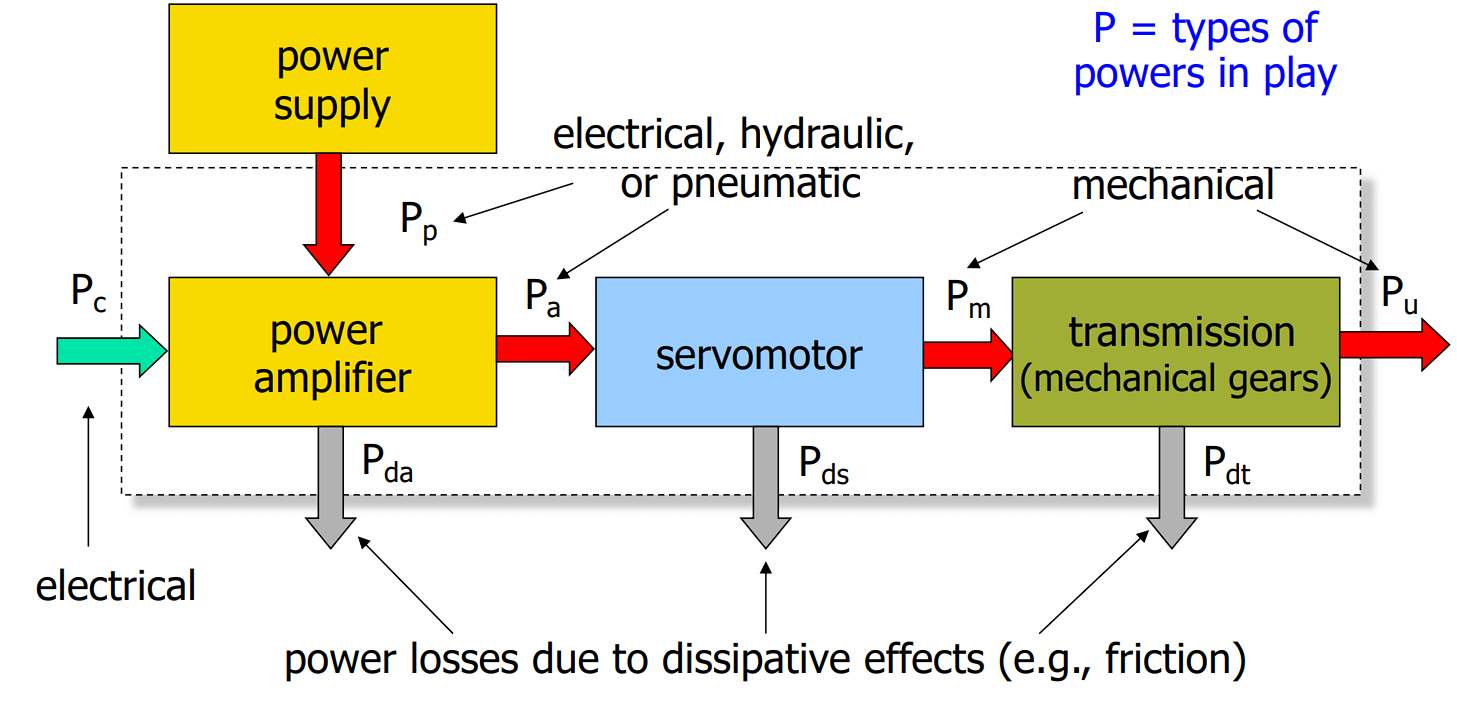
\includegraphics[width=0.7\textwidth ]{images/actuation_system.png} 
    \caption{Actuation system}
    \label{fig:Actuationsystem}
\end{figure}


We define the efficiency as the ratio between the output and input power:\begin{equation}
    \text{efficiency}=\frac{P_u}{P_c}.
\end{equation}
\section{Electrical Motors}
Since pneumatic system have difficulties to guarantee  high levels of precision, and the hydraulic actuation systems are expensive and needs hydraulic supply, in most of the cases electrical servo motors are mounted on the robots.\begin{itemize}
    \item advantages of electrical motors:\begin{itemize}
        \item power supply available everywhere
        \item low cost
        \item large variety of products
\item high power conversion efficiency
\item easy maintenance
\item no pollution in working environment
    \end{itemize}
    \item disadvantages\begin{itemize}
        \item overheating in static conditions (in the presence of gravity)
\item need special protection in flammable environments
\item some advanced models require more complex control laws
    \end{itemize}
\end{itemize}\begin{center}
    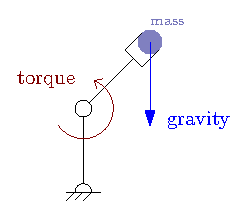
\includegraphics[width=0.25\textwidth ]{images/overheating.eps} 
\end{center}
If a robot should keep an object in a still position, the force of gravity tends to rotate the arms, so torque from the motors must be applied to keep that positions (this does not happen with hydraulic motors).
\begin{definition}
    A \textbf{servomotor} is a type of electric motor (AC or DC) specifically designed for the precision control of position, speed, and acceleration. It uses a closed-loop system with a feedback component (such as an encoder) that continuously monitors the motor's current position and compares it to the desired position. If there is a difference (an error signal), the controller corrects it, ensuring extremely accurate and dynamic motion.
\end{definition}
Desired characteristics for a servomotor mounted on a robot are:\begin{itemize}
    \item low inertia and high power-to-weight ratio
    \item high acceleration capabilities and large  range of operational velocities (1 to 2000 round per minute)
    \item low torque ripple\footnote{Torque ripple is an issue that arises in motors due to their construction, and it will be explained later.} and high accuracy in positioning
    \item power: 10 W to 10 kW.
\end{itemize}
There are two types of electrical motors\begin{itemize}
    \item Brushed DC: Has windings on the rotor (rotating part) and permanent magnets on the stator (stationary part). It uses physical brushes rubbing against a commutator to mechanically switch the current direction and maintain rotation.
    \item Brushless DC (BLDC): Has permanent magnets on the rotor and windings on the stator. It uses an electronic controller (instead of brushes/commutator) to electrically switch the current to the windings for rotation.
\end{itemize}\begin{center}
    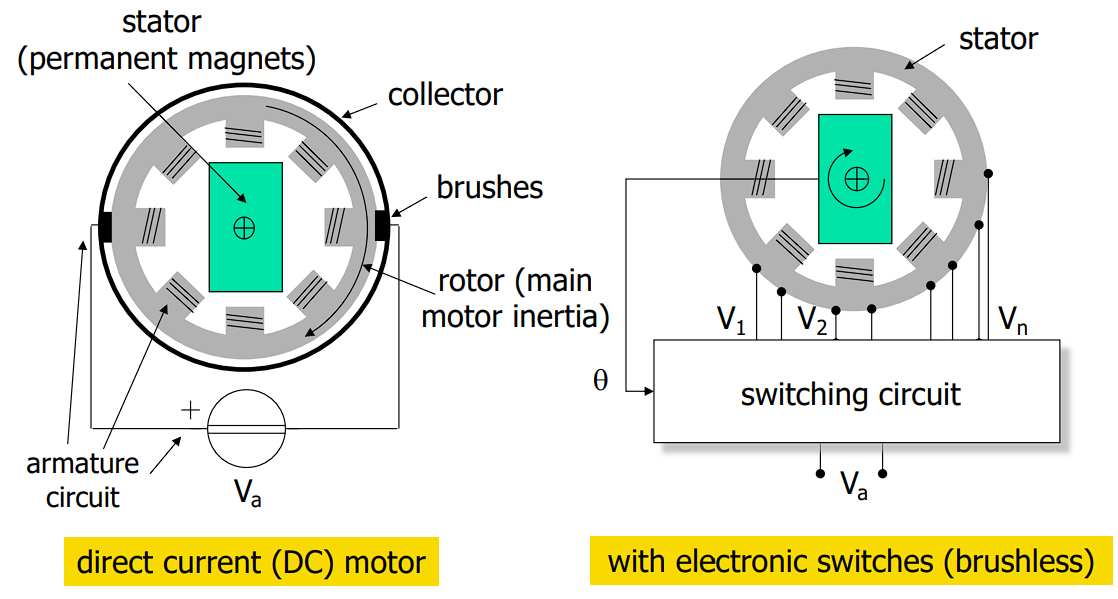
\includegraphics[width=0.7\textwidth ]{images/brush_brushless.png} 
\end{center}


The DC motor has a complex construction, but the mathematical model that describes it is simple. The rotor (the rotating part) includes copper windings (coils) through which current circulates in a determined direction; power is supplied thanks to the contact of brushes that rub against the motor. The entire assembly is immersed in a magnetic field provided by permanent magnets, as shown in figure \ref{fig:motor}.\bigskip

\begin{figure}[h!]
    \centering
    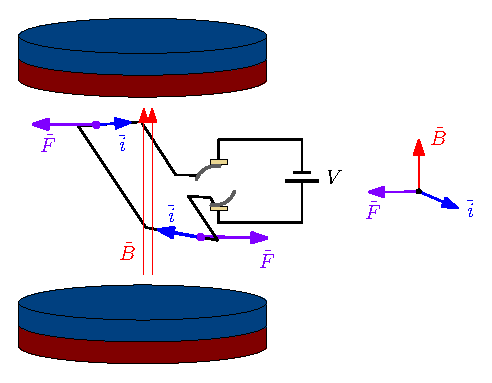
\includegraphics[width=0.6\textwidth ]{images/motore2.eps}
    \caption{brush DC motor}
    \label{fig:motor}
\end{figure}

The electrons will move in the direction of the vector  
$\bar i$
(current density), with intensity I, and due to the presence of a magnetic field  
$\bar B$, they will be subjected to the \textbf{Lorentz force}
\begin{equation}
     \bar F = I(\bar l \times \bar B)
\end{equation}
where $\bar l$ represents the section of wire.
In this way, a torque will be generated, causing the circuit to rotate. The brushes, colored yellow in figure \ref{fig:motor}, by making contact, ensure that the current circulates. Note how the slip ring is divided into two parts; it acts as a \textit{commutator}. This construction allows the current to reverse direction with every half-turn. If this were not the case, the Lorentz force would alternate, causing the rotor to oscillate until it stopped, without rotating, as shown in figure \ref{fig:commutazione}.\bigskip

\begin{figure}[h!]
    \centering
    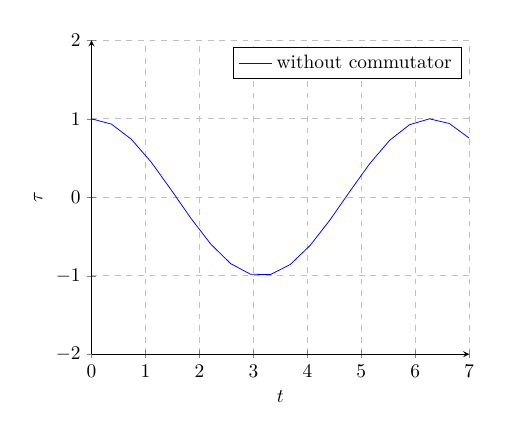
\begin{tikzpicture}[scale=0.7, transform shape]
        \begin{axis}[
        ymin=-2,
        ymax = 2,
        xmin=0,
        xmax = 7,
        axis lines = left,
        xtick distance=1, ytick distance=1,
        grid style=dashed,
        ymajorgrids=true,
        xmajorgrids=true,
        xlabel = \(t\),
        ylabel = {\(\tau\)},
        ]
        %Below the red parabola is defined
        \addplot [
        domain=0:7,
        samples=20,
        color=blue,
        ]
        {cos(deg(x))};
        \addlegendentry{without commutator}
        \end{axis}
        \end{tikzpicture}
        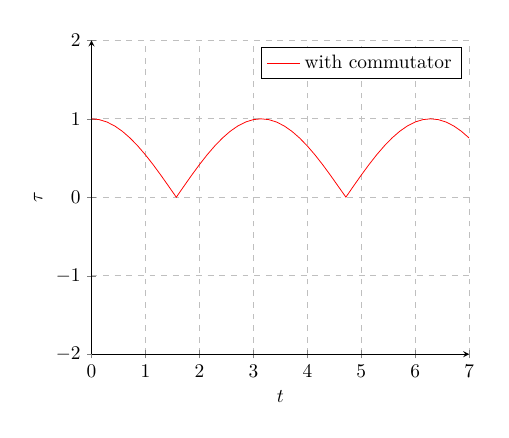
\begin{tikzpicture}[scale=0.7, transform shape]
        \begin{axis}[
        ymin=-2,
        ymax = 2,
        xmin=0,
        xmax = 7,
        axis lines = left,
        xtick distance=1, ytick distance=1,
        grid style=dashed,
        ymajorgrids=true,
        xmajorgrids=true,
        xlabel = \(t\),
        ylabel = {\(\tau\)},
        ]
        %Below the red parabola is defined
        \addplot [
        domain=0:7,
        samples=50,
        color=red,
        ]
        {abs(cos(deg(x)))};
        \addlegendentry{with commutator}
        \end{axis}
        \end{tikzpicture}
        \caption{Torque profile $\tau$}
        \label{fig:commutazione}
\end{figure}

\noindent The \textbf{torque} is equal to
\begin{equation}
    \bar T = (\bar r_1 \times  \bar F_1 + \bar r_2 \times  \bar F_2)
\end{equation}
We denote $\tau = \pm|\bar T|$ the \textit{scalar torque}.
\begin{center}
    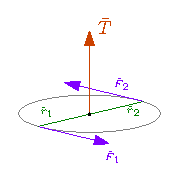
\includegraphics[width=0.25\textwidth ]{images/momento.eps}
\end{center}
The force $\bar F$  depends on the angle $\theta$ of the motor's rotation, because the change in the direction of the current  
$\bar i$
  can cause the force to attenuate. The torque becomes zero every time the angle between the generated force and the lever arm of rotation is $k\pi$, where $k\in\N$.

\begin{center}
    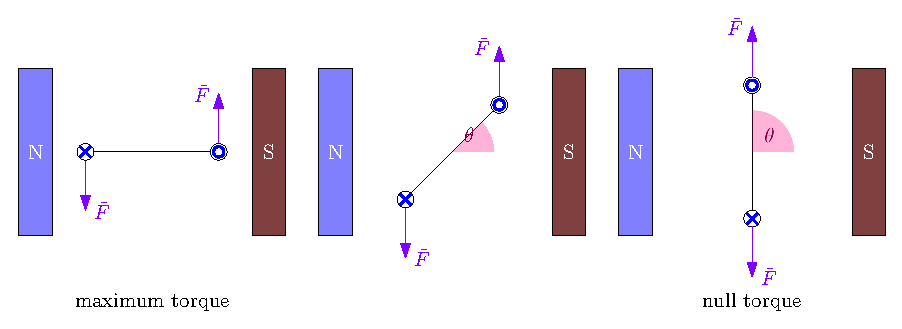
\includegraphics[width=1\textwidth ]{images/variazioneCoppia.eps}
\end{center}
\begin{center}
	\begin{tabular}{>{\centering\arraybackslash}m{3in}>{\arraybackslash}m{3in}}
        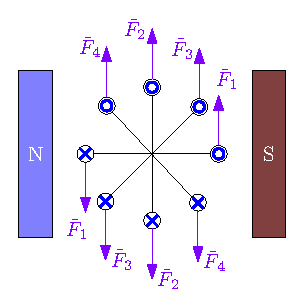
\includegraphics[width=0.33\textwidth ]{images/variazioneCoppia2.eps} & Because of this, the torque has an oscillatory behavior and is not constant; this phenomenon is called \textbf{torque ripple}. To limit this (and increase the torque), multiple coils can be added so that, at the instant one coil produces zero torque, another coil produces maximum torque.
		\\
	\end{tabular}
\end{center}
\begin{center}
    \begin{figure}[h!]
       \centering
       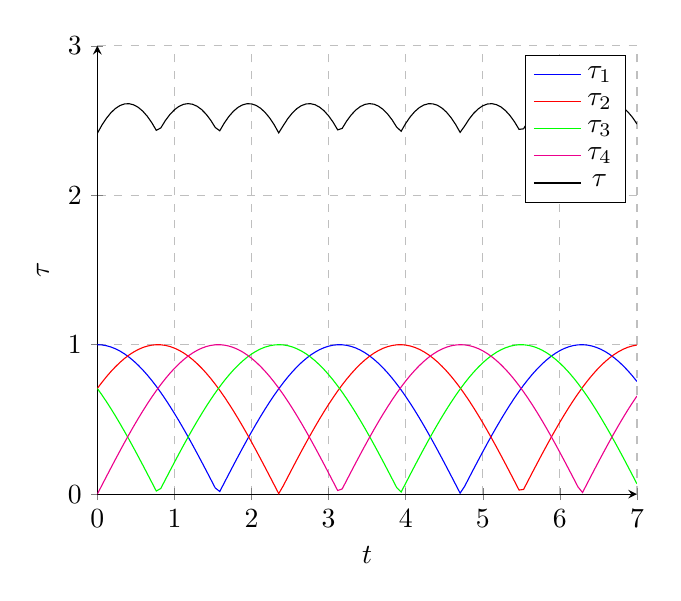
\begin{tikzpicture}[scale=1, transform shape]
           \begin{axis}[
           ymin=0,
           ymax = 3,
           xmin=0,
           xmax = 7,
           axis lines = left,
           xtick distance=1, ytick distance=1,
           grid style=dashed,
           ymajorgrids=true,
           xmajorgrids=true,
           xlabel = \(t\),
           ylabel = {\(\tau\)},
           ]
           %Below the red parabola is defined
           \addplot [
           domain=0:7,
           samples=120,
           color=blue,
           ]
           {abs(cos(deg(x)))};
           \addlegendentry{$\tau_1$}
           \addplot [
            domain=0:7,
            samples=120,
            color=red,
            ]
            {abs(cos((deg(x+((3/4)*pi)))))};
            \addlegendentry{$\tau_2$}
            \addplot [
            domain=0:7,
            samples=120,
            color=green,
            ]
            {abs(cos(deg(x+(pi/4))))};
            \addlegendentry{$\tau_3$}
            \addplot [
            domain=0:7,
            samples=120,
            color=magenta,
            ]
            {abs(cos(deg(x+(pi/2))))};
            \addlegendentry{$\tau_4$}
            \addplot [
            domain=0:7,
            samples=120,
            color=black,
            ]
            {abs(cos(deg(x+(pi/2))))+abs(cos(deg(x+(pi/4))))+abs(cos(deg(x+((3/4)*pi))))+abs(cos(deg(x)))};
            \addlegendentry{$\tau$}
           \end{axis}
           \end{tikzpicture}
           \caption{torque generated by multiple coils.}
        \end{figure}
    \end{center}
The greater the number of coils included, the more the torque ''flattens out'', tending towards a constant behavior.
\subsection{Dynamical Model of the Motor}
Now let's model an electric motor as a dynamical system. The motor is composed by two main sub-model\begin{itemize}
    \item An electromagnetic model 
    \item A mechanical model 
\end{itemize}
The commutator circuit have in series a resistor and an inductor, the model is shown in figure \ref{fig:model_motor}.

\begin{figure}[h!]
    \centering
    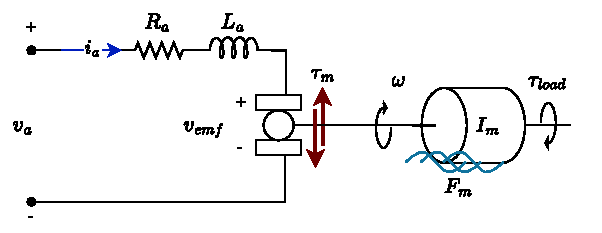
\includegraphics[width=0.8\textwidth ]{images/motor_scheme.drawio.pdf}
    \caption{Dynamical Model}
    \label{fig:model_motor}
\end{figure}

in the electromagnetic sub model, the voltage $v_a$ is given by the Kirchhoff laws\begin{equation}
    v_a(t)=R_ai_a(t)+L_a\frac{d i_a}{dt}+v_{emf}(t)
\end{equation}
where\begin{itemize}
    \item $R_a$ is the resistance coefficient 
    \item $L_a$ is the inductance. 
\end{itemize}
The term $v_{emf}(t)$ is called \textbf{Back Electromotive Force} and is a voltage generated within the rotating armature of an electric motor,  based on Faraday's Law of Induction, when the motor's armature coils $\omega(t)$ rotate and cut across the magnetic field (produced by the field coils or permanent magnets), a voltage is induced across the armature windings. Since a motor in motion is essentially acting as a generator, this is often called generator action. This voltage is proportional to the angular speed of the motor\begin{equation}\label{eq:model_balance_2}
    v_{emf}(t)=k_v\omega(t)
\end{equation}
Let's consider the mechanical sub model, we apply the newton law on torques, the scalar torque $\tau_m(t)$ of the rotating body is given by\begin{equation}
    \tau_m(t)=I_m\frac{d\omega}{dt}+F_m\omega(t)+\tau_{load}(t)
\end{equation}
where\begin{itemize}
    \item $I_m$ is the moment of inertia of the motor, a larger moment of inertia means the motor will take more torque and time to accelerate or decelerate to a given speed.
    \item $F_m$ is the viscous friction coefficient (since the motor never rotate in the void), and is proportional to the angular speed. It has a damping action on the rotational speed
    \item $\tau_{load}(t)$ is the external mechanical torque load given by the weight of the object that the motor is trying to rotate, and it opposes to the input torque.
\end{itemize}
The two sub models are related by an equation, it states that the torque $\tau_m$ of the motor is proportional to the applied current $i_a$ on the circuit:\begin{equation}\label{eq:model_balance}
    \tau_m(t)=k_ti_a(t)
\end{equation}
Let's define the state variables of our model, we can apply a voltage $v_a(t)$, and we are interested in the resulting angular position $\theta$ and speed $\dot\theta=\omega$.  \begin{align}
    &\begin{cases}
        \displaystyle v_a(t)=R_ai_a(t)+L_a\frac{d i_a}{dt}+v_{emf}(t)\\
        \displaystyle \tau_m(t)=I_m\frac{d\omega}{dt}+F_m\omega(t)+\tau_{load}(t)\\
    \end{cases}
\end{align}
by using the equations \eqref{eq:model_balance} and \eqref{eq:model_balance_2} we get
\begin{align}
    &\begin{cases}
        \displaystyle v_a(t)=R_ai_a(t)+L_a\frac{d i_a}{dt}+v_{emf}(t)\\
        \displaystyle k_ti_a(t)=I_m\frac{d\omega}{dt}+F_m\omega(t)+\tau_{load}(t)\\
    \end{cases}\implies \\ 
    &\begin{cases}
        \displaystyle L_a\frac{d i_a}{dt}=v_a(t)-R_ai_a(t)-k_v\omega(t)\\ 
        \displaystyle I_m\frac{d\omega}{dt}=k_ti_a(t)-F_m\omega(t)-\tau_{load}(t)\\
        \displaystyle \frac{d\theta}{dt}=\omega(t)
    \end{cases}
\end{align}
in the dot notation for derivatives:\begin{align}
   &\begin{cases}
        \displaystyle L_a\dot{i_a}=v_a(t)-R_ai_a(t)-k_v\omega(t)\\
        \displaystyle I_m\ddot\theta=k_ti_a(t)-F_m\omega(t)-\tau_{load}(t)\\
        \displaystyle \dot\theta=\omega(t)
    \end{cases}
\end{align}
the state variables are\begin{equation}
    \mathbf x  =\begin{pmatrix}
        \dot{i_a} \\ 
        \ddot \theta\\ 
        \dot \theta
    \end{pmatrix}
\end{equation}
the position $\theta$ can be found by integrating $\omega$. The motor is a system that given a input voltage over time $v_a(t)$, returns the electric current (more precisely, it's derivative, $i_a$ can be found by integrating over time), the angular speed  and the acceleration of the motor.\begin{center}
    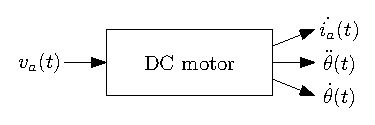
\includegraphics[width=0.4\textwidth ]{images/motor_abstract.eps}
\end{center}
\begin{quote}
    \textbf{About the notation}: if $f(t)$ is a function in the time domain, we denote $\mathcal L[f](s)=f(s)$ it's Laplace transform in the complex variable $s$. For example: \begin{equation}
        \mathcal L[i_a](s)=i_a(s)
    \end{equation}
\end{quote}
Let's analyze the model in the Laplace domain by considering the Laplace transform, and then draw the block diagram of the system. For the electrical model we have\begin{align}
    &\mathcal L\left[ \displaystyle L_a\dot{i_a}=v_a(t)-R_ai_a(t)-k_v\omega(t) \right]\implies\\ 
    &sL_a i_a(s)=v_a(s)-R_ai_a(s)-k_v\omega(s)\implies\\
    &sL_a i_a(s)+R_ai_a(s)=v_a(s)-k_v\omega(s) \implies \\
    &(sL_a+R_a)i_a(s)=v_a(s)-k_v\omega(s) \implies\\
    &i_a(s)=\frac{v_a(s)-k_v\omega(s)}{sL_a+R_a}
\end{align}
assuming that the quantities are null in $t=0$. In the end, we get:\begin{equation}
    i_a(s)=\frac{v_a(s)-k_v\omega(s)}{sL_a+R_a}
\end{equation}
$v_a$ and $v_{emf}$ are external input to the model, so the transfer function for the electromagnetic sub model is\begin{equation}
    \frac{1}{sL_a+R_a}
\end{equation}
\begin{center}
    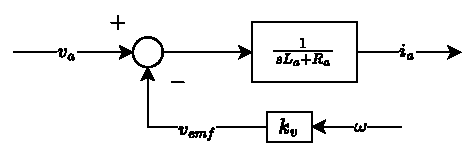
\includegraphics[width=0.7\textwidth ]{images/EM_model.drawio.pdf}
\end{center}
By analogous steps, we find that the transfer function for the mechanical sub model is\begin{equation}
    \frac{1}{sI_m+F_m}
\end{equation}
where the input is the torque $\tau_m$ from which we subtract the torque load $\tau_{load}$.
\begin{center}
    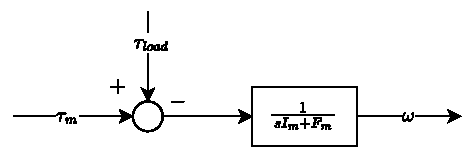
\includegraphics[width=0.7\textwidth ]{images/Mech_model.drawio.pdf}
\end{center}
We can chain the models since $\tau_m=k_ti_a$\begin{center}
    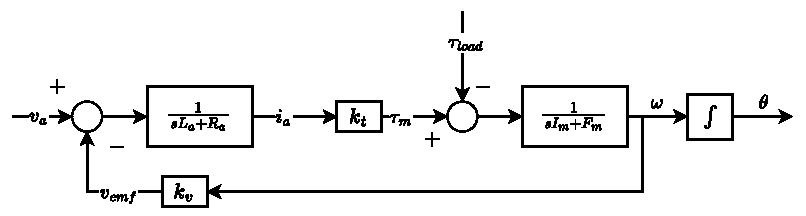
\includegraphics[width=1\textwidth ]{images/full_model.drawio.pdf}
\end{center}\begin{proposition}
    The two constants $k_v$ and $k_t$ are equals\begin{equation}
        k_v=k_t.
    \end{equation}
\end{proposition}
\textit{Proof}: This is trivially true. The electric power generated by the EM sub model is\begin{equation}
    v_{emf}i_a
\end{equation}
the mechanical power is\begin{equation}
    \tau_m\omega 
\end{equation}
since the conservation of power holds in energy transformations:\begin{equation}
    v_{emf}i_a= \tau_m\omega
\end{equation}
applying equations \eqref{eq:model_balance_2},\eqref{eq:model_balance} we get\begin{align}
    &v_{emf}i_a= \tau_m\omega\implies\\ 
    &k_v\omega i_a= k_ti_a\omega\implies \\ 
    &k_v=k_t. 
\end{align}
\hfill$\blacksquare$
\section{Transmissions}
\redText{TODO}
\section{Sensors}
\redText{TODO}
\chapter{Direct Kinematics}
\section{Position and Orientation of a Rigid Body}
We have a base reference frame $RF_A=(\mathbf x_A,\mathbf y_A,\mathbf z_A)$, and a rigid body $B$ in the space, let's say that there is a fixed reference frame $RF_B=(\mathbf x_B,\mathbf y_B,\mathbf z_B)$ attached to a point of $B$, a vector ${}^A\mathbf p\in\R^3$ can describe the position of the whole body respect to the frame $RF_A$, and a $3\times3$ matrix is sufficient to describe the orientation of that body.
\begin{center}
    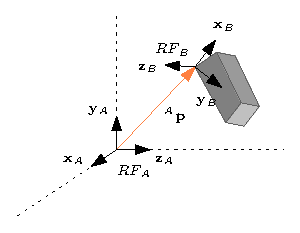
\includegraphics[width=0.5\textwidth ]{images/rigid_body_pose.eps}
\end{center}
The orientation of the reference frame $RF_B$ respect to $RF_A$ is described by a matrix $R$ of the following type\begin{itemize}
    \item $R$ is orthonormal, the columns vector are orthogonal from each other and have unitary length. 
    \item $R^T=R^{-1}\implies RR^T=I$
    \item $\det R=1$
\end{itemize}
These are the matrices in the orthogonal group $SO(3)$. More precisely, we denote ${}^AR_B$ the matrix that describe the orientation of $RF_B$ respect to $RF_A$. \begin{equation}
    {}^AR_B=\begin{pmatrix}
        &&\\
        {}^A\mathbf x_B&{}^A\mathbf y_B&{}^A\mathbf z_B\\
        &&
    \end{pmatrix}
\end{equation}
the components of ${}^AR_B$ are the direction cosines of the axes of $RF_B$ with respect to $RF_A$. In general, let's say the reference vector of two different frames are\begin{align}
    (\mathbf x_A,\mathbf y_A,\mathbf z_A)\\
    (\mathbf x_B,\mathbf y_B,\mathbf z_B)
\end{align}
the matrix ${}^AR_B$ are the following\begin{equation}
    {}^AR_B=\begin{pmatrix}
        \mathbf x^T_A\mathbf x_B&\mathbf x^T_A\mathbf y_B&\mathbf x^T_A\mathbf z_B\\ \\
        \mathbf y^T_A\mathbf x_B&\mathbf y^T_A\mathbf y_B&\mathbf y^T_A\mathbf z_B\\ \\
        \mathbf z^T_A\mathbf x_B&\mathbf z^T_A\mathbf y_B&\mathbf z^T_A\mathbf z_B
    \end{pmatrix}
\end{equation}
since all the basis vectors are unitary, and\begin{equation}
    \mathbf u^T\mathbf v=\|\mathbf u\|\cdot\|\mathbf v\|\cdot\cos\alpha
\end{equation}
we have that each component represent the angle between the two considered axis.
\begin{center}
    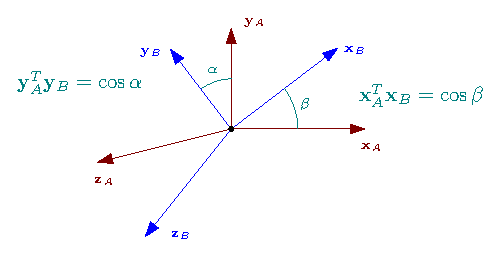
\includegraphics[width=0.6\textwidth ]{images/orientation_reference.eps}
\end{center}
for three different reference frame $RF_i,RF_j,RF_k$, the \textbf{chain rule} holds:\begin{equation}
    {}^kRF_i{}^iRF_j={}^kRF_j
\end{equation}
so, if ${}^A\mathbf p$ is a vector in the frame reference $RF_A$, the same vector in the reference frame $RF_B$ is\begin{equation}
    {}^B\mathbf p={}^BRF_A{}^A\mathbf p
\end{equation}
so the matrix is used for the \textbf{change of coordinates} between the two frames with different orientation.\begin{center}
    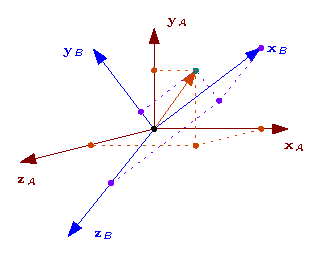
\includegraphics[width=0.5\textwidth ]{images/coordinate_change.eps}
\end{center}
The position of a rigid body can be expressed in cartesian, cylindrical or spherical coordinates. A point in $\R^3$ in cylindrical coordinates is described by\begin{equation}
    r,\theta,h 
\end{equation}
where the transformation from cylindrical to cartesian is\begin{align}
    &x=r\cos\theta\\
    &y=r\sin\theta\\
    &z=h 
\end{align}
the inverse transformation (assuming $r\ge 0$) is\begin{align}
    &r=\sqrt{x^2+y^2}\\ 
    &\theta =\text{atan2}(y,x)\\
    &h=z
\end{align}
The atan2$(y, x)$ function is a two-argument arctangent that returns the angle $\theta$ in standard position whose terminal side passes through the point $(x, y)$, correctly placing the angle in the correct quadrant ($\pi$ to $\pi$ or $0$ to $2\pi$). Is defined as follows;\begin{equation}
    \text{atan2}(y, x) =
\begin{cases}
\text{atan}\left(\frac{y}{x}\right) & x > 0 \\
\pi + \text{atan}\left(\frac{y}{x}\right) & y \geq 0, x < 0 \\
-\pi + \text{atan}\left(\frac{y}{x}\right) & y < 0, x < 0 \\
\frac{\pi}{2} & y > 0, x = 0 \\
-\frac{\pi}{2} & y < 0, x = 0 \\
\text{undefined} & y = 0, x = 0
\end{cases}
\end{equation}
We saw that the rotation matrices can describes the change of coordinates between two frames, and the orientation of a given frame with respect to another. These matrices can also describes the rotation of a vector in $\R^3$, let's consider a rotation around the $z$ axis. We have a vector $\mathbf v$ that lies in the $xy$ plane, with coordinates $$\mathbf v=\begin{pmatrix}
    x\\ 
   y\\z
\end{pmatrix}=\begin{pmatrix}
    \|\mathbf v\|\cos\alpha\\ 
    \|\mathbf v\|\sin\alpha\\z
\end{pmatrix}$$
where $\alpha$ is the angle between $\mathbf v$ and the $x$ axis. We rotate $\mathbf v$ by $\theta$ radiant around the $z$ axis, obtaining a new vector $\mathbf v'$ with coordinates$$
\mathbf v'=\begin{pmatrix}
    \|\mathbf v\|\cos(\alpha+\theta)\\ 
    \|\mathbf v\|\sin(\alpha+\theta)\\z
\end{pmatrix}=\begin{pmatrix}
    x\cos\theta-y\sin\alpha\\ 
    x\sin\theta+y\cos\alpha\\z
\end{pmatrix}
$$\begin{center}
    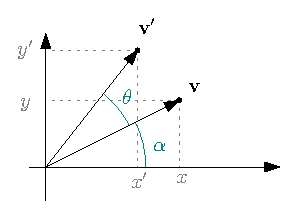
\includegraphics[width=0.35\textwidth ]{images/rotation_around_z.eps}
\end{center}
Notice how the relation between $\mathbf v$ and $\mathbf v'$ is given by a matrix $ \mathbf v'=R_z(\theta)\mathbf v$ called the \textbf{elementary rotation around $z$} by $\theta$ radiant.\begin{equation}
    R_z(\theta) =\begin{pmatrix}
        \cos\theta & -\sin\theta&0\\
        \sin\theta&\cos\theta&0\\
        0&0&1
    \end{pmatrix} 
\end{equation}
similarly, are defined elementary rotation around $x$ and $y$ too:\begin{equation}
     R_x(\theta) =\begin{pmatrix}
        1&0&0\\
        0&\cos\theta & -\sin\theta\\
        0&\sin\theta&\cos\theta
    \end{pmatrix}  \ \ \ \ \  
    R_y(\theta) =\begin{pmatrix}
        \cos\theta&0&\sin\theta\\ 0&1&0\\ -\sin\theta&0&\cos\theta
    \end{pmatrix} 
\end{equation}
So an orthonormal matrix have 3 possible interpretations:\begin{itemize}
    \item it can describe the orientation of a rigid body with respect to a reference frame
    \item it can describe the change of coordinates between two different frames one rotated respect to the other
    \item it can describe the rotation operator on a vector.
\end{itemize}
\subsubsection{Example}
Let's consider a sphere of radius $1$ as a rigid body, we have a reference frame $RF_S$ for the sphere fixed in the center, clearly the top pole in that frame is in position ${}^S\mathbf p=\begin{pmatrix}
    0&1&0
\end{pmatrix}^T$.\begin{center}
    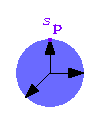
\includegraphics[width=0.1\textwidth ]{images/sphere.eps}
\end{center}
We have a base frame $RF_0$ with the canonical base
$\mathbf e_x,\mathbf e_y,\mathbf e_z$, the sphere is placed in position $\begin{pmatrix}
    3&3&0
\end{pmatrix}^T$, we denote ${}^0\mathbf s$ the position of the frame $RF_S$ respect to $RF_0$. The sphere, is also rotated by 90 degrees clock wise around the $z$ axis.\begin{center}
    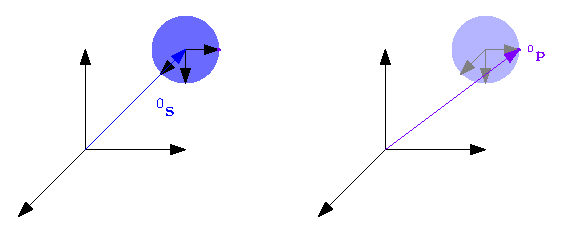
\includegraphics[width=0.7\textwidth ]{images/sphere_2.eps}
\end{center}
to find the position of the north pole $\mathbf p$ respect to $RF_0$, we have to apply the rotation matrix $R_z(-\nicefrac{\pi}{2})$ to ${}^S\mathbf p$ and consider the translation.
\begin{align}
    &{}^0\mathbf p=R_z(-\nicefrac{\pi}{2}){}^S\mathbf p+{}^0\mathbf s=\\
&\begin{pmatrix}
        0 & 1&0\\
        -1&0&0\\
        0&0&1
    \end{pmatrix} \begin{pmatrix}
    0\\1\\0
\end{pmatrix}+\begin{pmatrix}
    3\\3\\0
\end{pmatrix}=\begin{pmatrix}
    4\\3\\0
\end{pmatrix}.
\end{align}
\end{document}